\newcommand{\source}[1]{\caption*{Source: {#1}} }

\section{Verwandte Arbeiten}\raggedbottom

\subsection{Semantische Segmentierung im medizinischen Bereich}

\subsubsection{Semantische Segmentierung}

Die semantische Segmentierung erfolgt in drei Schritten:

Klassifizierung: Klassifizierung eines bestimmten Objekts im Bild.

Lokalisieren: Auffinden des Objekts und Zeichnen eines Begrenzungsrahmens um das Objekt.

Segmentierung: Gruppierung der Pixel in einem lokalisierten Bild durch Erstellung einer Segmentierungsmaske.

Im Wesentlichen kann man die Aufgabe der semantischen Segmentierung als Klassifizierung einer bestimmten Bildklasse und deren Abgrenzung von den übrigen Bildklassen durch Überlagerung mit einer Segmentierungsmaske bezeichnen.

Veranschaulicht spricht man von einer Klassifizierung der Bildern auf Pixelebene.

\subsubsection{Medizinischer Bereich}

Die medizinische Bildgebung umfasst viele Kategorien, von 2- und 3 dimensionalen MRT Scans des Herzens, Gehirns und des Magen-Darm Trakts, 2 dimensionalen Röntgen Bildern sowie Ausschnitte aus der Videoendoskopie.

Bereits in den 90er Jahren wurde sich mit Segmentierungsarchitekturen auseinandergesetzt und Baselines geschaffen. Zu dieser Zeit lieferten Methoden im Bereich Mustererkennung die besten Ergebnisse. Die Autoren legten viel Wert auf Datenvorverarbeitung und werteten die zu jener Zeit besten Architekturen aus. Damals griff man auf einen erweiterungs-basierten Ansatz zurück, es wurde mit Algorithmen wie
\href{https://en.wikipedia.org/wiki/K-nearest_neighbors_algorithm}{kNN},
\href{https://en.wikipedia.org/wiki/Maximum_likelihood_estimation}{Maximum Likelihood} und
\href{https://en.wikipedia.org/wiki/Eigenvalues_and_eigenvectors}{Characteristic vector} experimentiert.

Trotz aller Bemühungen wiesen die Modelle nur eine Genauigkeit von 3\% bis 34\% auf. \citet{Clarke:Mri1995}

Jedoch waren die Autoren davon überzeugt, dass maschinelle Segmentierung eine wichtige Rolle im Bereich der Verarbeitung von MRT Daten darstellen wird. Mit wachsender Akzeptanz auf klinischer Seite sowie dem allgemeinen technischen Fortschritt sollen akkurate Segmentierungen von MRT Bildern im Livebetrieb möglich werden.

\newpage

\subsection{Deep Learning-Techniken für die Segmentierung medizinischer Bilder:
Errungenschaften und Herausforderungen}

Dank der immensen Verbesserung der Rechenleistung der Hardwareeinheiten wurde das Thema Deep Learning immer interessanter und gehört heutzutage zur Standard Vorgehensweise im Bereich Computer Vision. Architekturen wie das U-Net \citet{U-Net} haben sich hierbei im medizinischen Bereich besonders bewiesen. Im Verlauf der Jahre nach der Veröffentlichung in 2015 sind viele wissenschaftliche Arbeiten mit die er Erweiterungen der Grundarchitektur vorstellten, so dass es heute ein breites Spektrum an Modellen gibt, die an verschiedene (medizinische) Problemstellungen angepasst sind. \citet{Hesamian}

\subsection{Intelligentes Zuschneiden des Inputs}

Dimitrios G. Zaridis et al. \citet{SmartCrop} haben sich ebenfalls mit verschiedenen State-of-the-Art U-Net Architekturen auseinandergesetzt und jene als Baseline für ihre Arbeit genutzt. Trotz der beachtlichen Leistung, die die Modelle lieferten, waren sie der Meinung dass noch Verbesserungspotential vorhanden ist. Sie fanden heraus, dass das Vorhandensein eines Klassenungleichgewichts, in dem der Anteil der Hintergrundpixel dem Anteil der zu segmentierenden Klasse überwiegt, zu Problemen bei der Genauigkeit der Vorhersage führen kann. 

Mithilfe einer auf Deep Learning aufbauenden Architektur haben die Autoren es geschafft, dieses Klassenungleichgewicht zu reduzieren, in dem ein Neuronales Netzwerk die gesuchten Organe lokalisiert, das Originalbild zuschneidet um am Ende das Verhältnis von Vorder- und Hintergrundpixeln bestmöglich zu normalisieren. Dies führte bei einem Großteil der getesteten Modelle zu einem erheblichen Anstieg der Genauigkeit, die Ergebnisse von U-Net+ und ResU-Net++ verbesserten sich um bis zu 8\%.

\section{Grundlagen}\raggedbottom

\subsection{Magen-Darmtrakt}

Für das Gewinnen von Erkenntnissen sowie der Analyse des Datensatzes ist es von nöten, ein anatomisches Grundverständnis von der Körperregion zu besitzen, den sie beschreiben. Oben angefangen beginnt es mit dem Magen, der unten am Dickdarm abschließt und davon umgeben ist der Dünndarm (vergl. Abb \ref{Fig:magen-darm-trakt}). 

Beim Datensatz handelt es sich um segmentierte MRT-Bilder von anonymisierten Patienten die am UW-Madison Carbone Cancer Center behandelt wurden. Beim Magen- und Darmtrakt handelt es sich um einen selbst für Menschen schwer zu segmentierenden Bereich aufgrund seiner Komplexität, seiner unregelmäßigen Formen sowie variierender Position der Organe (Vergl. \cite{Chen_2020}).

\begin{figure}[H]
   \begin{minipage}{0.48\textwidth}
     \centering
     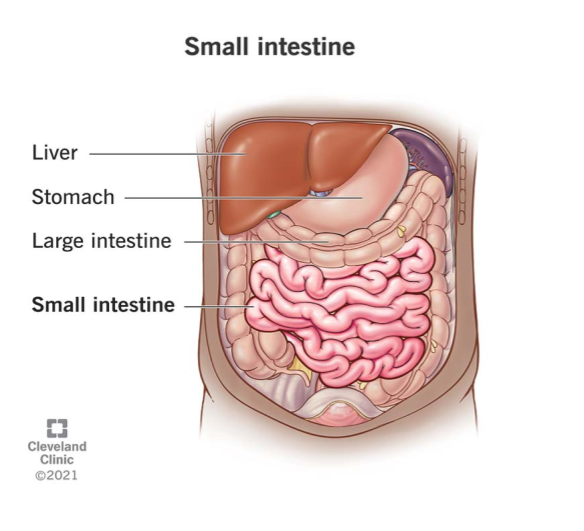
\includegraphics[width=1\linewidth]{bilder/intestines}
     \caption{Magen-Darm Trakt. Stomach, large intestine und small intestine stehen jeweils für Magen, Dick- und Dünndarm. }
   \end{minipage}\label{Fig:magen-darm-trakt}
   \hfill
   \begin{minipage}{0.48\textwidth}
     \centering
     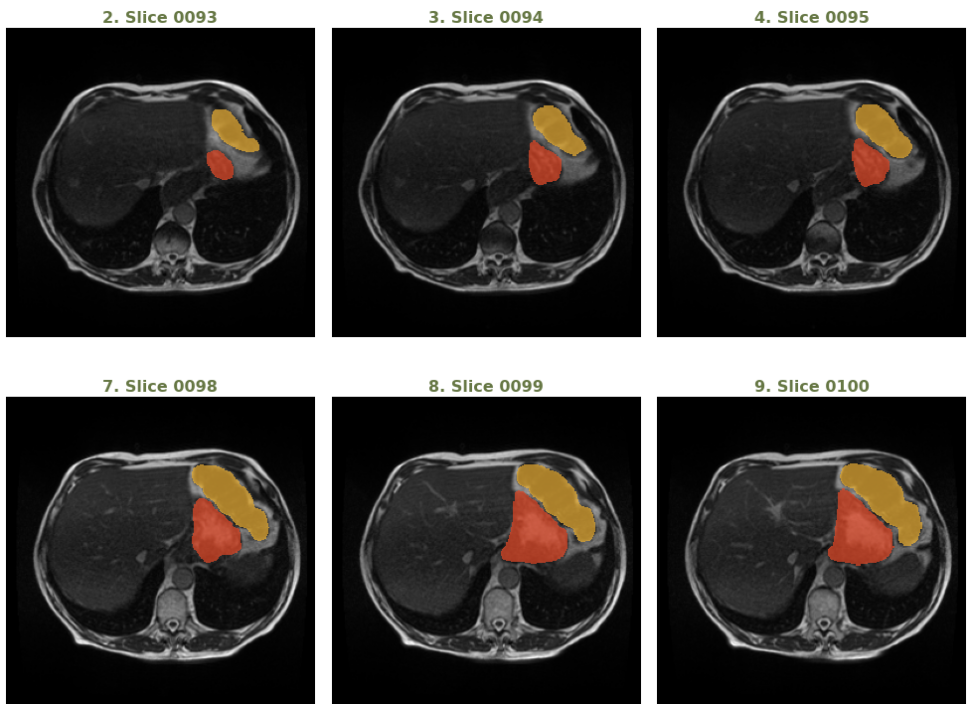
\includegraphics[width=1\linewidth]{LaTex/bilder/beispieldaten.png}
     \caption{ Zu sehen ist hier eine Abfolge von segmentierten Teilstücken eines Falles. Die rote Markierung beschreibt den Magen, die orangene den Dickdarm.}
   \end{minipage}\label{Fig:magen-mrt}
\end{figure}

\subsection{Kaggle} \label{ssec:kaggle}

Diese Arbeit baut auf der 
\href{https://www.kaggle.com/competitions/uw-madison-gi-tract-image-segmentation/overview/description}{UW-Madison GI Tract Image Segmentation}
Challenge auf, die von der University of Wisconsin Carbone Cancer Center Pancreas Pilot Research Grant organisiert wurde und von denen die Daten auch bereitgestellt wurden.

Ziel ist es eine Architektur zu finden, die dazu in der Lage ist zukünftig Onkologen im Klinikalltag dabei zu helfen, Tumore besser und schneller zu lokalisieren um so eine genauere Strahlentherapie durchführen zu können. 

Im Rahmen des Wettbewerbs wurden die Daten anhand einer Mischung aus dem Dice-Koeffizienten zu 40\% (Vergl. \ref{ssec:dc}) sowie der Hausdorff-Metrik zu 60\% (Vergl. \ref{ssec:hdorff}) auf ungesehenen Testdaten von ungefähr 50 Personen ausgewertet, siehe  \href{https://www.kaggle.com/competitions/uw-madison-gi-tract-image-segmentation/data}{hier}.

\subsection{U-Net}
% CNN, Convolution, Maxpooling oder ReLu erklären?

U-Net wurde im Jahr 2015 von Olag Ronneberger et al. \citet{U-Net} vorgestellt als Segmentierungsarchitektur für den biomedizinischem Bereich und bildet die Baseline dieser Arbeit. Neu in der Herangehensweise ist der Encoder-Decoder Part, die dem Netzwerk ermöglicht räumliche Merkmale zu lernen.

Klassisch handelt es sich beim Encoder um ein
\href{https://en.wikipedia.org/wiki/Convolutional_neural_network}{Convolutional Neural Network} (CNN) , bestehend es aus 5 bis 6 downsampling Schichten und der gleichen Menge an  upsampling Schichten im Decoder Part. 

Eine downsample Operation besteht zum einen aus einer
\href{https://en.wikipedia.org/wiki/Convolution}{Convolution Operation}
sowie einer
\href{https://computersciencewiki.org/index.php/Max-pooling_/_Pooling}{Max Pooling}
an deren Ende jeweils eine
\href{https://deepai.org/machine-learning-glossary-and-terms/relu}{ReLu}
 Aktivierungsfunktion zum Einsatz kommt. In diesem Schritt lernt das Modell Eigenschaften auf Pixelebene, wie zum Beispiel Formen, Ecken, Kanten. Hierbei halbieren sich die Eingabedimensionen und die Tiefe des Bildes wird erhöht. 

Im Decoder wird das Bild wieder auf seine ursprüngliche Größe mittels 
\href{https://en.wikipedia.org/wiki/Deconvolution}{Transpose Convolution operations}
gebracht. Hier ersetzt die transponier Operation die Max Pooling Operation \autoref{Fig:unet-diagram}. 

Durch die Kombination aus En- und Decoder ist es möglich, Bilder semantisch zu segmentieren. Den Output des Modells bildet eine Maske, bestehend aus Nullen und Einsen, die der Eingabegröße gleicht und bestenfalls den Wert Eins an der Stelle der gesuchten Klasse enthält.

\begin{figure}[H]
	\begin{center}
		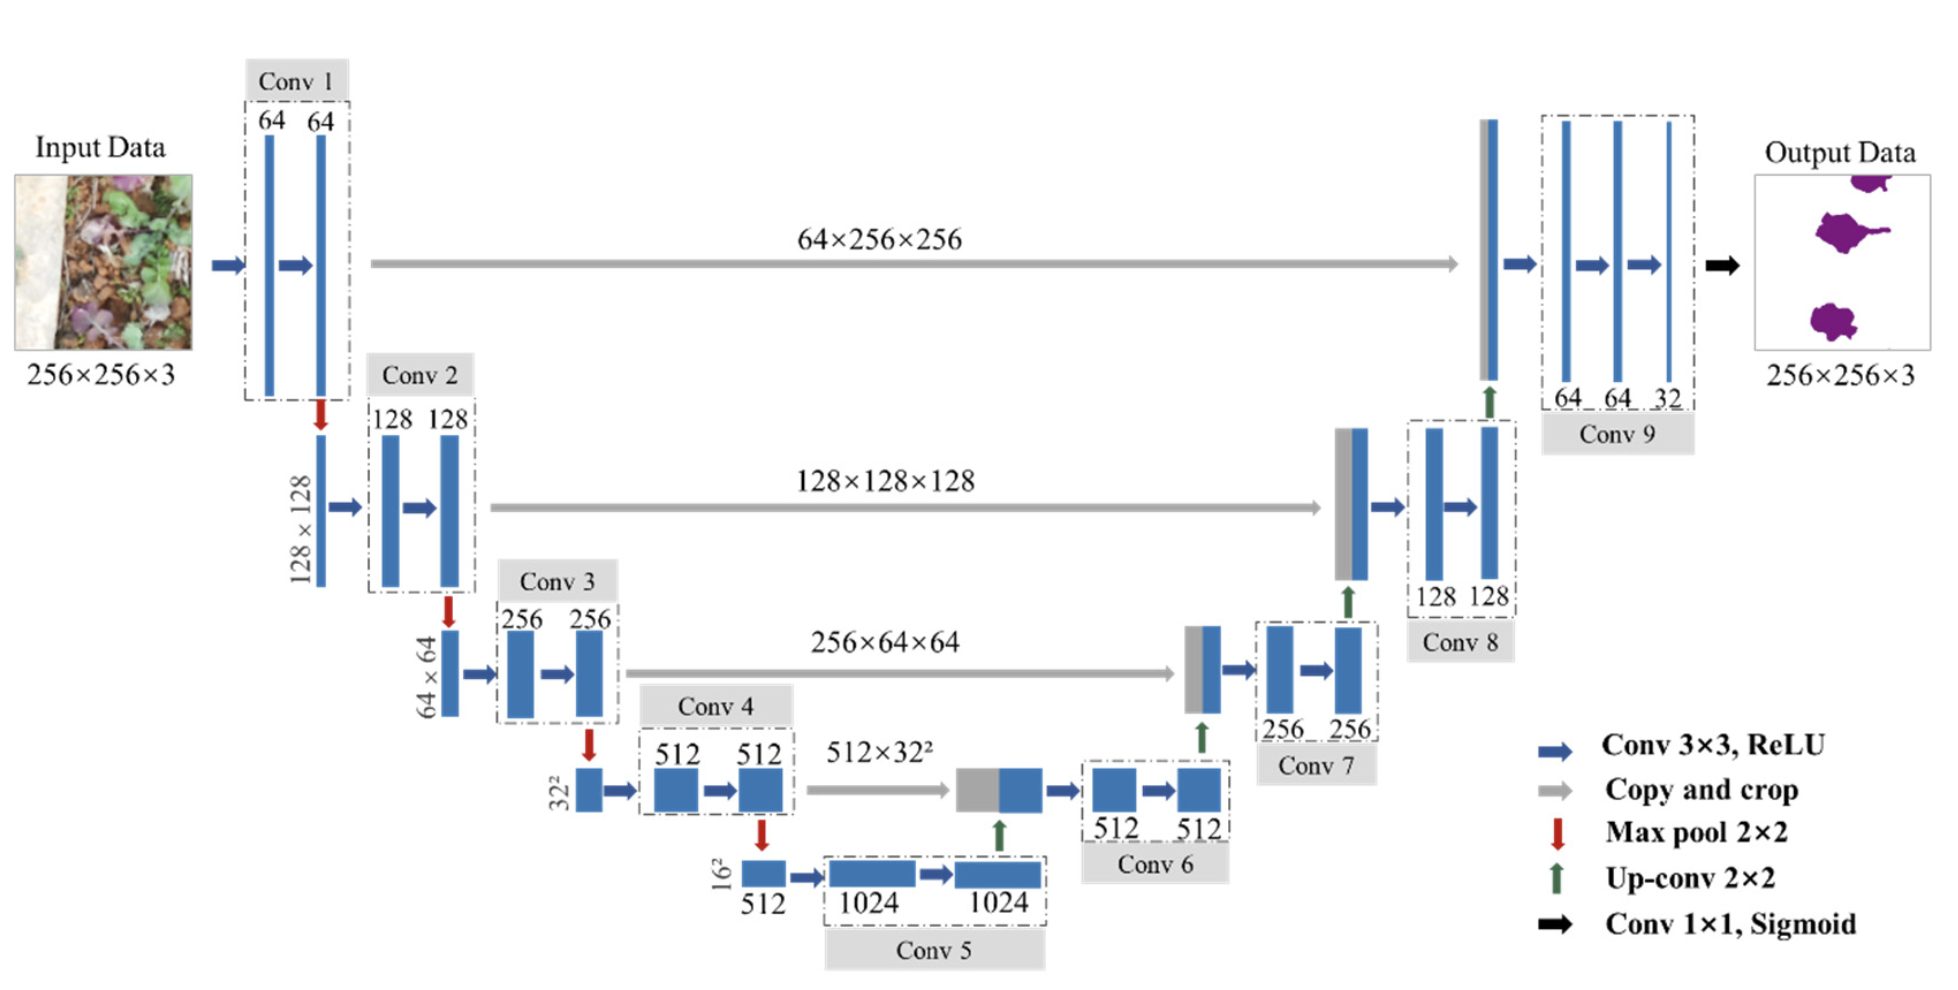
\includegraphics[width=430pt]{bilder/u-net-architecture}
		\caption{U-Net Architektur \citet{Zhang:2020}}\label{Fig:unet-diagram}
	\end{center}
\end{figure}


\subsection{EfficientNet}
EfficientNet ist eine von Google zusammengestellte Sammlung an CNN's. Klassisch verbessert man die Genauigkeit eines CNN's mittels dem Erhöhen der Netzwerkdimensionen, wie der Breite oder der Tiefe. Tan et al. verfolgen einen neuen Ansatz, sie skalieren den Input in all seinen Dimensionen - mittels einem Compound Koeffizienten und geht dabei einem Schema nach, im Gegensatz zur klassischen Methode, wo Skalierungen willkürlich vorgenommen werden. \autoref{Fig:compund-scaling}

Verglichen mit anderen state-of-the-art Modellen weist EfficientNet eine höhere Genauigkeit bei stark verringerter Anzahl an Parametern auf, was ein Resultat der generalisierten Skalierungsmethode ist. Es besteht aus acht Architekturen, EfficientNet-B0 bildet die Basis und ist vergleichbar mit dem \citet{MobileNetV2}.


\begin{figure}[H]
	\begin{center}
		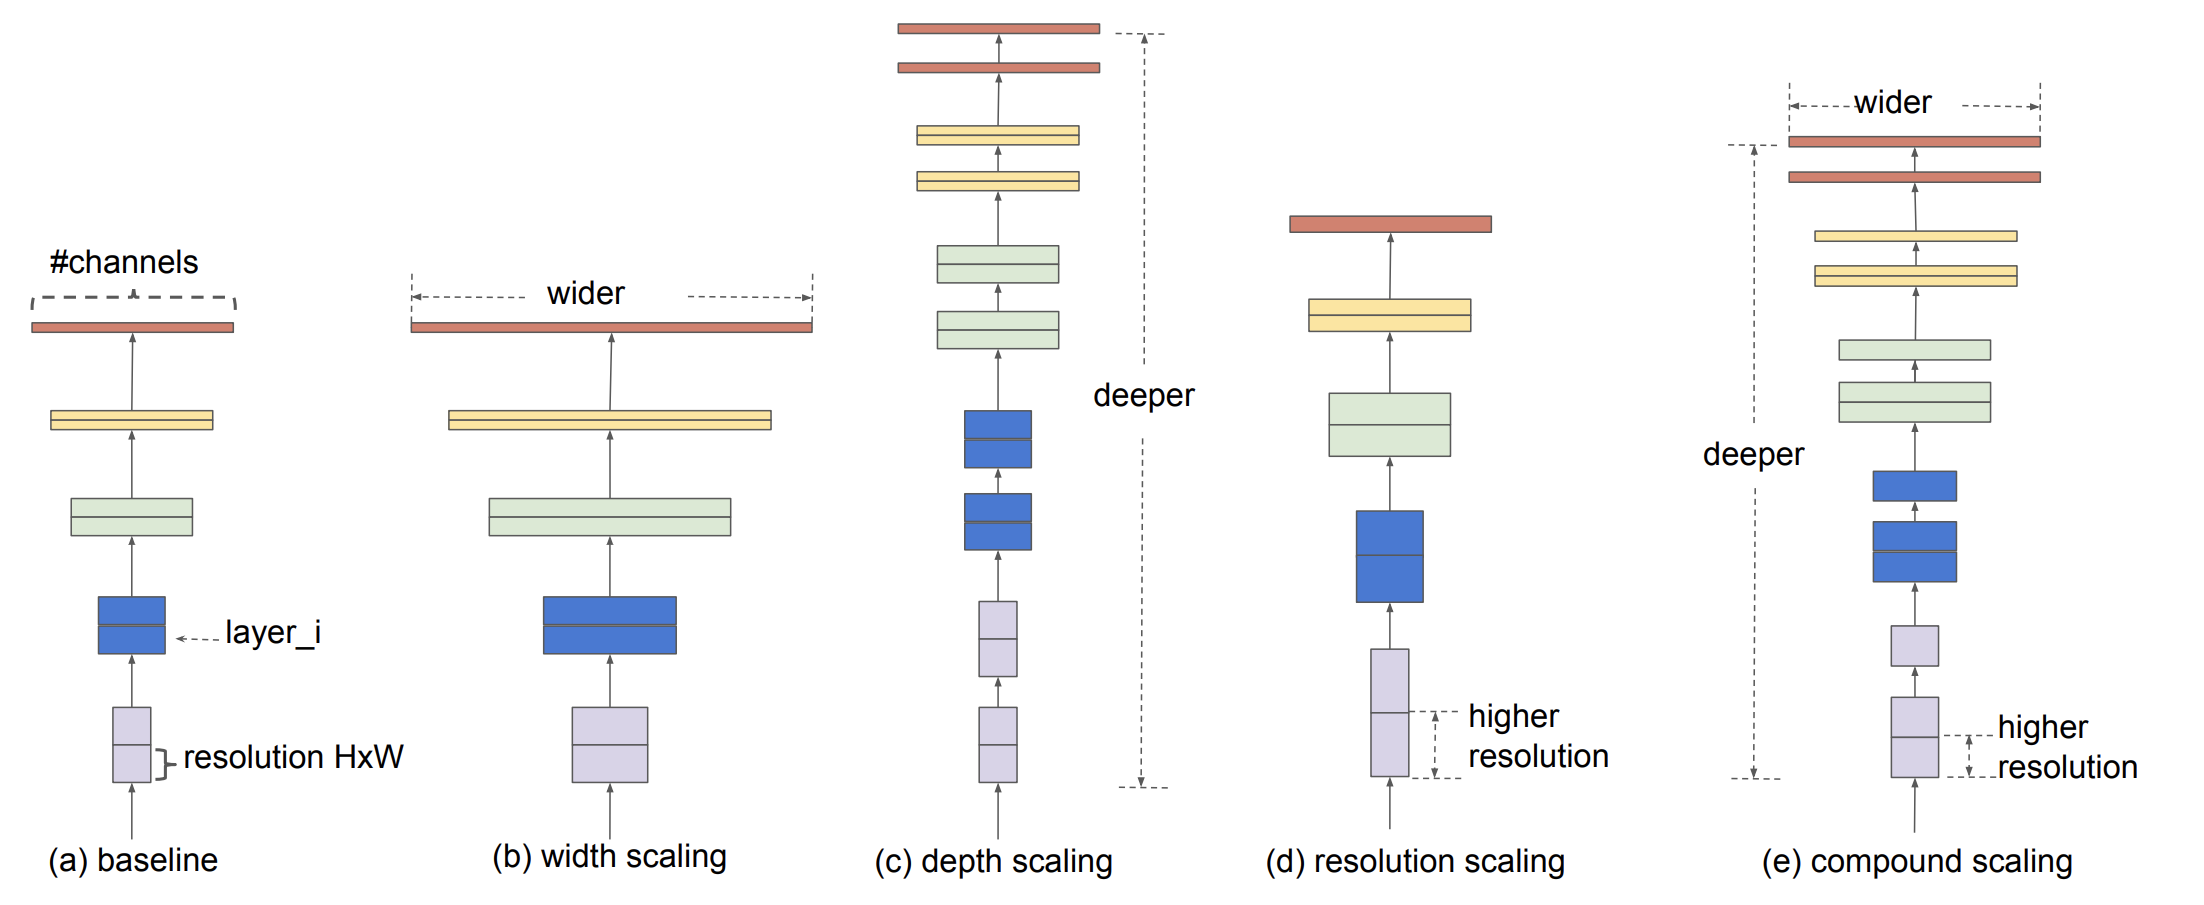
\includegraphics[width=430pt]{bilder/efficientnet}
		\caption{Veranschaulischung des Skalierungskoeffizienten (d), der alle Dimensionen gleichzeitig und gleichmäßig behandelt. (Tan et al. \citet{EfficientNet}) }\label{Fig:compund-scaling}
	\end{center}
\end{figure}



\section{Methodik}\raggedbottom

\subsection{Datenanalyse}

Im Folgenden beziehen sich die Werte {X} immer auf auf die Vorhersage und {Y} auf die Groundtruth.

\begin{table}[H]
	\begin{center}
	        \small
	        \setlength\tabcolsep{2pt}
		\begin{tabular}{|c|c|c|c|c|c|c|c|c|}
			\hline
			Index  & ID & Class & Segmentation \\
			\hline \hline
			1     & case134\textunderscore day0\textunderscore slice\textunderscore 0085 	& large\textunderscore bowel 	&  NaN  \\
			2     & case134\textunderscore day0\textunderscore slice\textunderscore 0085 	& small\textunderscore bowel 	&  41591 5 41599 7 41949 27 ...  \\
			3     & case134\textunderscore day0\textunderscore slice\textunderscore 0085 	& stomach 	&  NaN \\
			4     & case123\textunderscore day0\textunderscore slice\textunderscore 0001 	& large\textunderscore bowel 	&  35223 6 74352 7 32312 12 ...   \\
			5     & case123\textunderscore day0\textunderscore slice\textunderscore 0001 	& small\textunderscore bowel 	&  63432 5 12354 7 41949 12 ...  \\
			6     & case123\textunderscore day0\textunderscore slice\textunderscore 0001 	& stomach 	&  NaN \\
			\hline
		\end{tabular}
		\caption{Beispieldaten für zwei Slices}\label{tabelle_daten}
	\end{center}
\end{table}

Der Datensatz besteht aus 85 verschiedenen Patienten, davon hat jeder 3 bis 5 Tage MRT-Bildmaterial. Der 3 dimensionale Scan eines jeden Tages ist aufgeteilt in 144  bzw. in seltenen Fällen 80 Teilstücken. Demnach verfügt jeder Patient über ein Kontigent an 80 bis 720 Bildern.

115 488 Zeilen und enthält drei Features: ID, Klasse und einem Run-lenght codierten String, der die Maske enthält. \autoref{tabelle_daten}. Jeder ID sind drei Zeilen gewidmet, jeweils den Klassen für Dick- Dünndarm und Magen. Zu jeder ID existiert ein Graustufenbild, welche sich im train Ordner befinden, ein Beispiel der Ordnerhierarchie ist hier zu sehen (Vergl. Abb. \ref{Fig:train-data}).

\begin{figure}[H]
	\begin{center}
		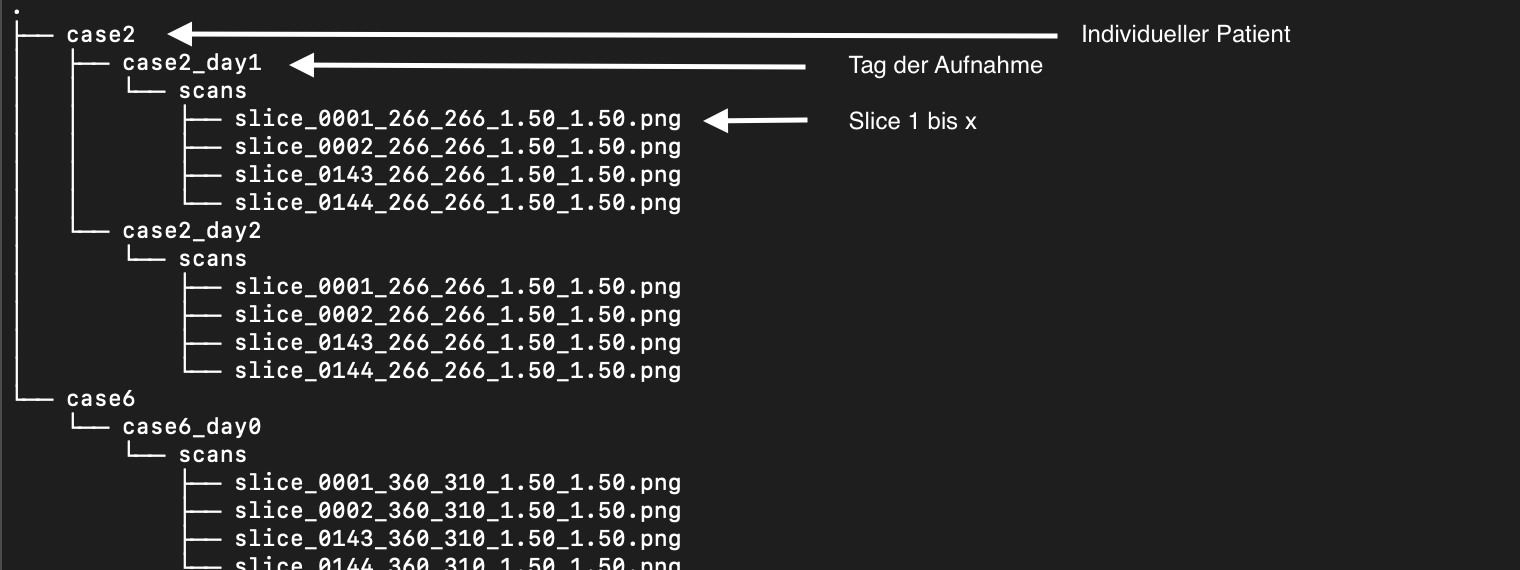
\includegraphics[width=350pt]{bilder/data_tree}
		\caption{Ordnerstruktur der Trainingsdaten. Slice 1 ist das unterste und 144 das oberste Teilstück der 3d Aufnahme.}\label{Fig:train-data}
	\end{center}
\end{figure}

Jedes Teilstück besitzt vier Werte im Namen (z.B. 266\textunderscore 266\textunderscore 1.50\textunderscore 1.50.png), die ersten beiden stehen für die Auflösung des Bildes und die letzten beiden für den physischen Abstand der Pixel in Millimeter. Der Großteil der Aufnahmen stammt von Tag Null und belaufen sich auf 11 680 (Vergl. Abb. \ref{Fig:pie-chart}. Die darauf meisten Teilstücke hat Tag 20, betrachtet man die Verteilung und schließt den 0. Tag aus findet man eine Normalverteilung vor (Vergl. Abb. \ref{Fig:slice_per_day}

\begin{figure}[H]
   \begin{minipage}{0.48\textwidth}
     \centering
		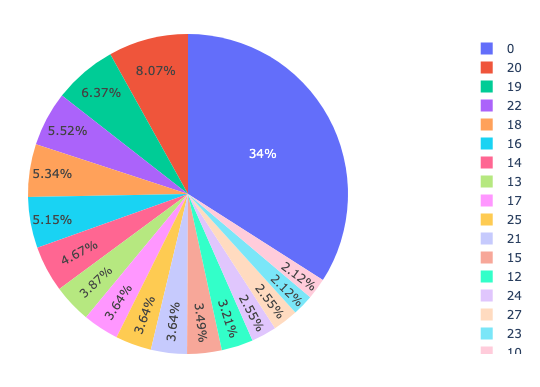
\includegraphics[width=1\linewidth]{LaTex/bilder/day_slice_pie.png}
		\caption{Verhältnis der Verteilung der Teilstücke an verschiedenen Tagen.}\label{Fig:pie-chart}
   \end{minipage}\hfill
   \begin{minipage}{0.48\textwidth}
     \centering
     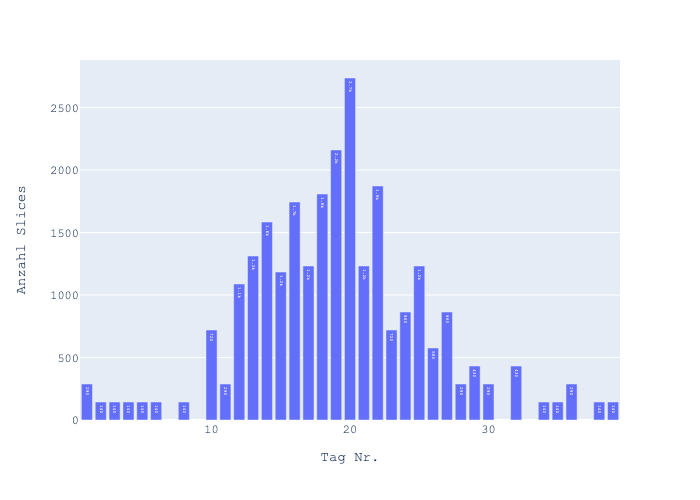
\includegraphics[width=1.2\linewidth]{LaTex/bilder/day_slice.png}
     \caption{Verteilung der Teilstücke ohne Tag 0.}\label{Fig:slice_per_day}
   \end{minipage}
\end{figure}

Beim betrachten der Verteilung der Segmentierungen fällt auf, dass das Vorkommen für jede Klasse stark variiert, am häufigsten sind gar keine segmentierten Teilstücke. 

\begin{table}[!ht]
    \centering
    \begin{tabular}{|c|c|c|c|}
    \hline
        Dickdarm & Dünndarm & Magen & Ohne \\ \hline
        37\% & 29\% & 22\% & 56\% \\ \hline
    \end{tabular}
    \label{Tab:klassenverteilung}
\end{table}

\subsection{Bildgröße} \label{ssec:input-size}

Es handelt sich bei den Trainingsdaten um relativ kleine Bilder. Es sind vier verschiedene Größen im Datensatz vorhanden, die rechteckigen Exemplare stammen in Anbetracht der Pixelwerte sehr wahrscheinlich von einem anderem MRT-Gerät.

\begin{table}[!ht]
    \centering
    \begin{tabular}{|c|c|c|c|c|}
    \hline
        Größe & 234 {x} 234 & 266 {x} 266 & 276 {x} 276 & 310 {x} 360 \\ \hline
        Anteil in \% & 0.37\% & 67.34\% & 3.12\% & 29.17\% \\ \hline
        \varnothing Pixelwert & 1145 & 1005 & 1148 & 134 \\\hline
    \end{tabular}
    \label{Tab:klassenverteilung}
\end{table}



\subsection{Metadatenextraktion}

Anhand der ID eines jedes Slices war es möglich verschiedene Metadaten dem originalem Dataframe zu hinzuzufügen. Außerdem ist jede ID nun einzigartig vorhanden und enthält alle drei Klassen in der selben Zeile. \autoref{tabelle_meta_daten}

% & rs & re & cs & ce & count & path00 & path01 & path02 & image\textunderscore paths

\begin{table}[H]
 \begin{center}
  \resizebox{\textwidth}{!}{
   \begin{tabular}{|l|l|l|l|l|l|l|l|l|l|l|l|l|l|}
     \hline
     Idx  & ID &  large\textunderscore bowel & small\textunderscore bowel & stomach & case & day & slice & path & width & height & pixel\textunderscore x & pixel\textunderscore y \\
     \hline \hline
     1     & case134\textunderscore day0\textunderscore slice\textunderscore 0085 	& NaN & 41591 5  ...    & NaN & 134 & 0 & 85 & input\textbackslash  & 266 & 266 & 1.5 & 1.5  \\
     2     & case134\textunderscore day0\textunderscore slice\textunderscore 0086 	& 41591 27 ... & NaN    & NaN & 134 & 0 & 86 & input\textbackslash  & 266 & 266 & 1.5 & 1.5  \\
     3     & case134\textunderscore day0\textunderscore slice\textunderscore 0086 	& NaN & NaN   & NaN & 134 & 0 & 87 & input\textbackslash  & 266 & 266 & 1.5 & 1.5  \\
     \hline
   \end{tabular}}
   \caption{Metadaten von dreier Teilstücke}\label{tabelle_meta_daten}
 \end{center}
\end{table}


\subsection{Vorarbeit}

\subsubsection{2.5 dimensionale Daten} \label{ssec:semi3d-data}

Klassisch haben die Slices die Dimensionen 
\begin{equation}
H \times W \times 1
\end{equation}
da es sich um Graustufenbilder handelt. U-Net arbeitet klassisch aber mit RGB Bildern, also einem 3 Channel Input
\begin{equation}
H \times W \times 3
\end{equation}
somit ist die Idee, aufeinanderfolgende Slices mit einem bestimmten Stride (Abstand) zu Verketten und dem Input so mehr Tiefe zu geben.

\begin{figure}[H]
	\begin{center}
		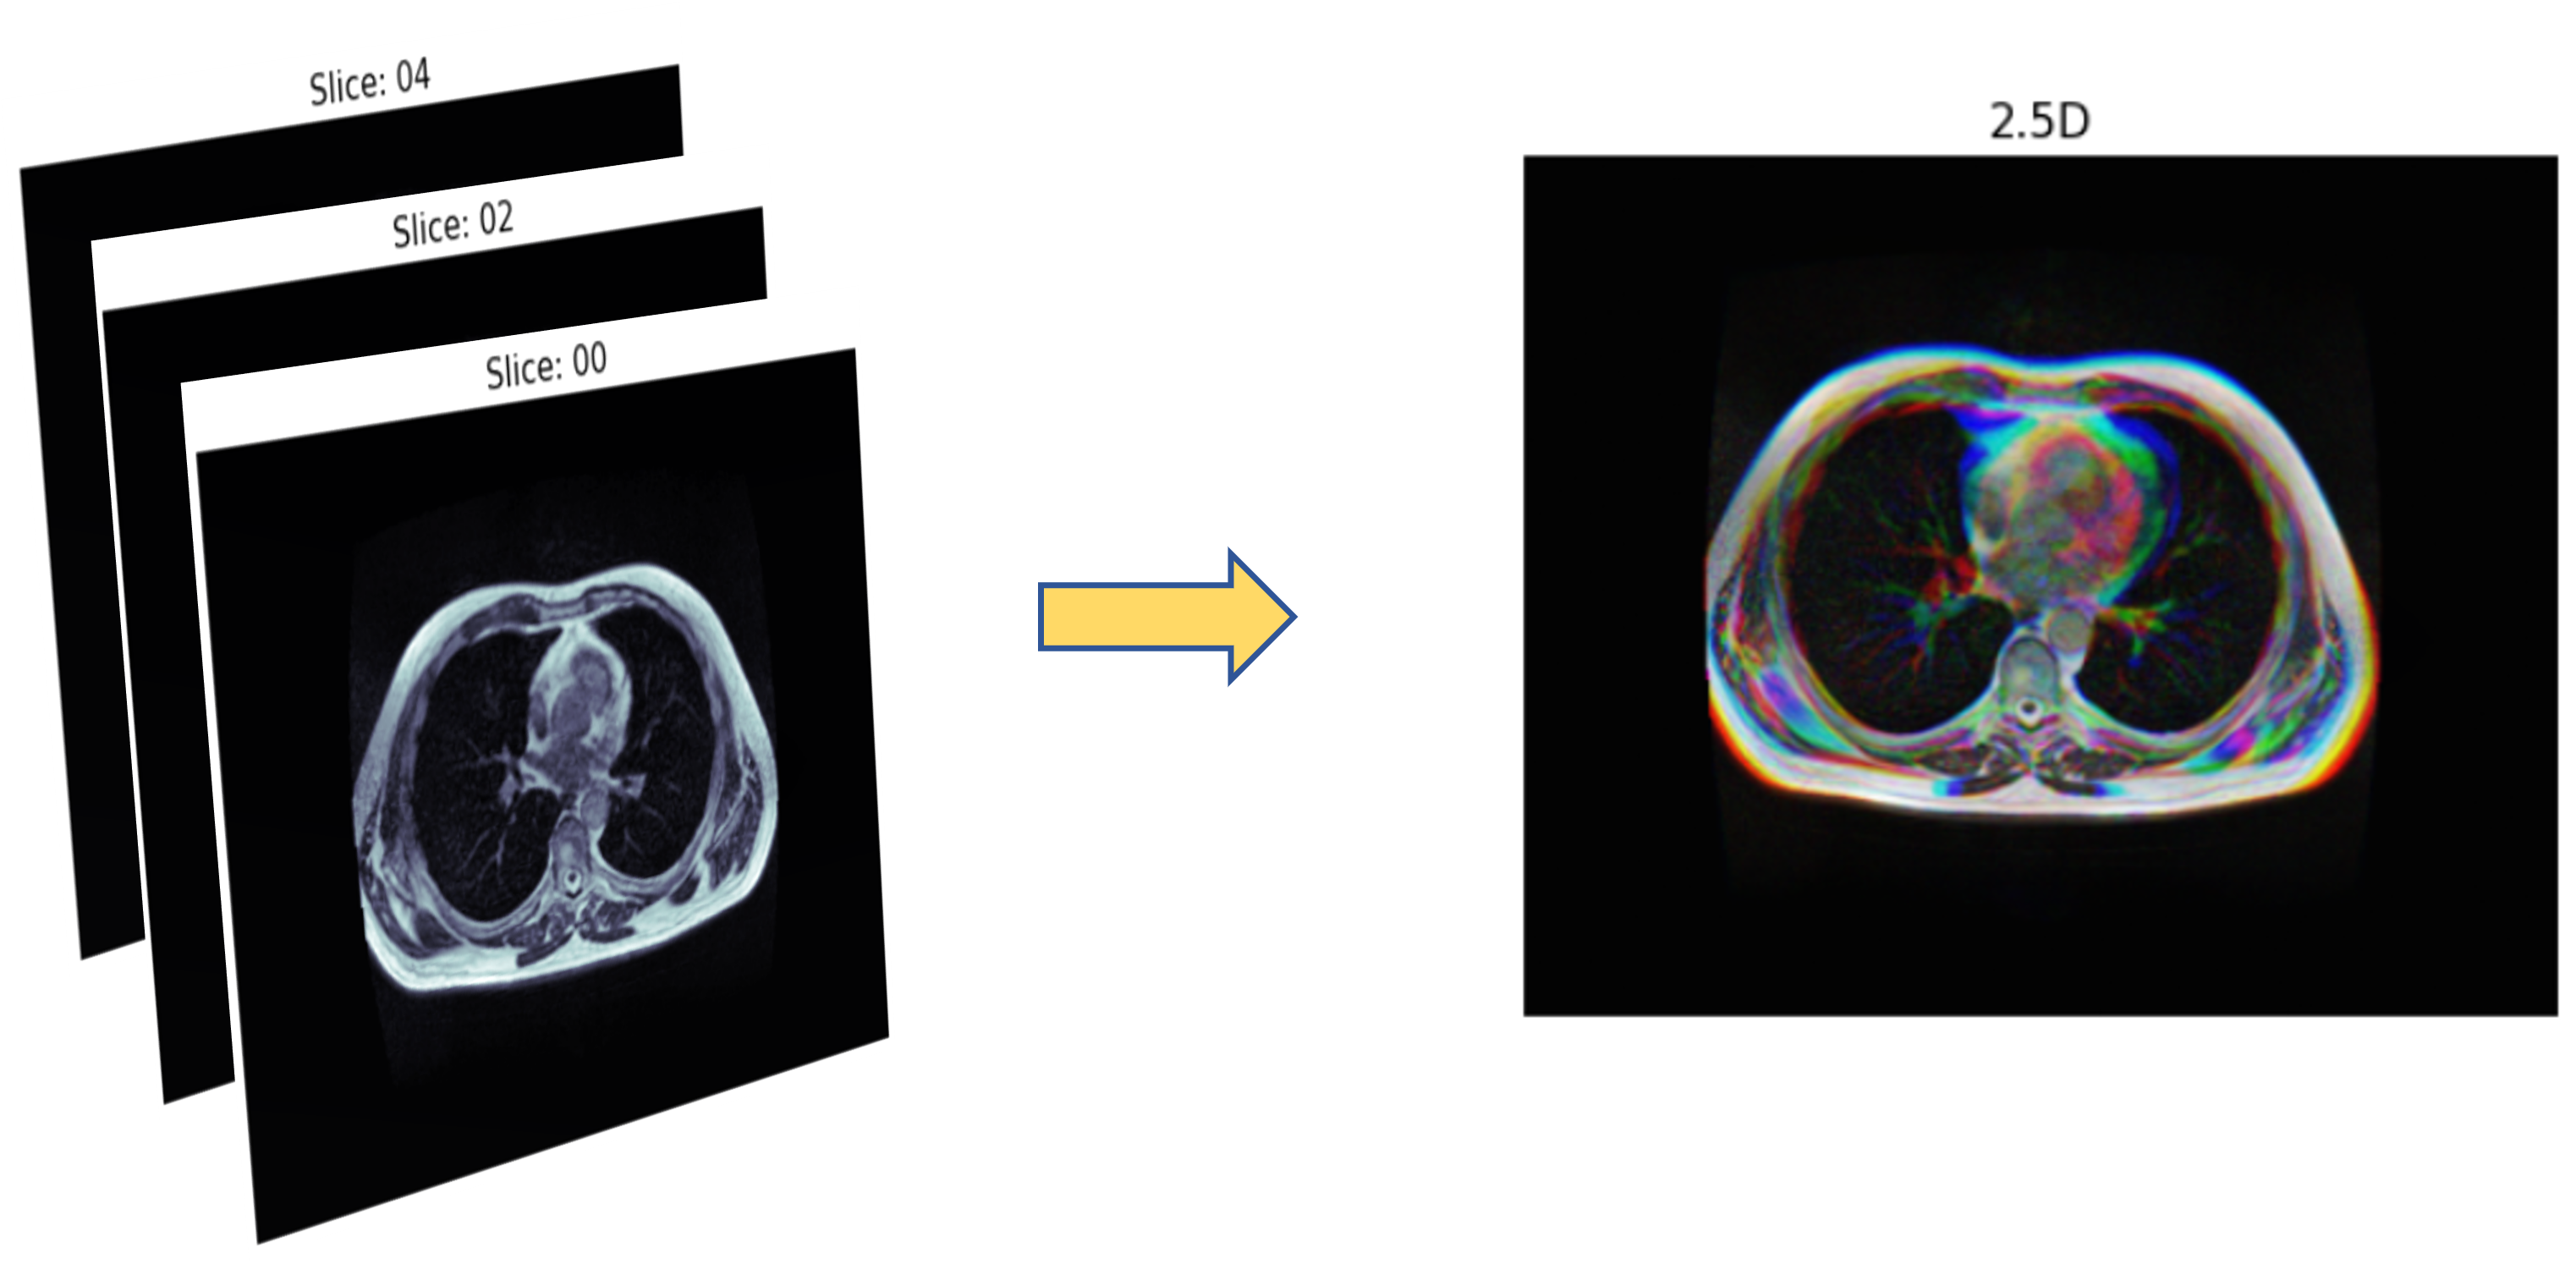
\includegraphics[width=350pt]{bilder/25d_input}
		\caption{Semi-3-dimensionaler Input \href{https://www.kaggle.com/competitions/uw-madison-gi-tract-image-segmentation/discussion/322549}{2.5 Dim Data}}\label{Fig:25d-data}
	\end{center}
\end{figure}

Diese Methode hat gegenüber 3 dimensionalen Daten einige Vorteile: es wird weniger Rechenleistung benötigt, die Trainingspipeline muss nur minimal angepasst werden, die Auswertung bleibt ebenfalls gleich und die Daten können jedem Modell übergeben werden, welche darauf ausgelegt sind RGB Bilder zu segmentieren. \cite{Chen_2020} haben damit ebenfalls ihr Modell erweitert und ihre Ergebnisse verbessert, bevor sie zu 3 dimensionalen Daten übergingen.

\subsubsection{Intelligentes Zuschneiden} \label{ssec:intellicrop}

Ein bekanntes Problem bei der Segmentierung von Organen anhand von MRT-Bildern ist das starke Klassenungleichgewicht zwischen Hintergrund- und Vordergrundpixeln (In diesem Fall Dickdarm, Dünndarm und Magen). \citet{SmartCrop} untersuchten dieses Problem und waren dazu in der Lage, das Ungleichgewicht zu mindern und die Performance zu erhöhen. 

Die Eingabebilder wurden für jeden Tag pro Fall individuell zugeschnitten. Zu beginn wird das Hintergrundrauschen mit einem Medianfilter beseitigt, um das kleinste Rechteck aus der Menge zu finden, welches den Wertebereich enthält, der ungleich null ist. Dieser Prozess wird für jedes Teilstück aus dem Tag wiederholt und das kleinste Rechteck welche alle Bilder aus jenem Fall und Tag berücksichtigt wird zurückgegeben und den Metadaten der Trainingsdaten hinzugefügt.

Anschließend werden die Werte dem Trainingsdatensatz hinzugefügt. Ein Beispiel von Case 134, Tag 21, Slice 70 ist hier zu sehen: \autoref{tab:crop_table} 

\begin{table}[H]
 \begin{center}
  \scalebox{1.1}{
\begin{tabular}{|l|l|l|l|l|l|l|}
\hline
 ID & Case & Day & RS & RE & CS & CE \\ \hline
 1 & 134 & 21 & 84 & 10000 & 0 & 359 \\ \hline
 2 & 113 & 22 & 50 & 10000 & 0 & 332  \\ \hline
\end{tabular}
}
\caption{Ausschnitt aus der Zuschnitt-Tabelle.}\label{tab:crop_table}
 \end{center}
 \end{table}
 
 RS, RE, CS und CE stehen in diesem Kontext für Zeilenanfang und Ende sowie Spaltenanfang und Ende. Im Dataloader wurden die Bilder dann zur Traningszeit zugeschnitten.
 
 So konnte das Ungleichgewicht für jede Klasse gesunken werden (Werte wurden gerundet): 

\begin{table}[H]
\centering
\begin{tabular}{|l|c|c|}
\hline
Klasse & ohne Zuschnitt & mit Zuschnitt \\ \hline
Dickdarm & 144 & 134\\ \hline
Dünndarm & 158 & 146 \\ \hline
Magen & 286 & 265\\ \hline
Total & 60 & 56\\ \hline
\end{tabular}
\caption{\label{tab:ratio}Verhältnis von Vorder- zu Hintergrundpixeln}
\end{table}

\begin{figure}[H]
    \begin{minipage}{0.45\textwidth}
    \centering
    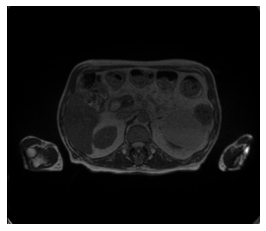
\includegraphics[width=1\linewidth]{LaTex/bilder/orig.png}
    \caption{Originalbild mit Maßen 310 x 360}
    \end{minipage}\hfill
    \begin{minipage}{0.45\textwidth}
    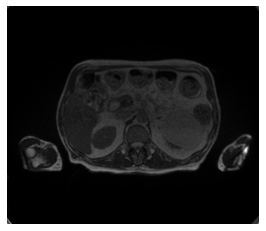
\includegraphics[width=1\linewidth]{LaTex/bilder/crop.png}
    \caption{Zugeschnittenes Teilstück mit Maßen 220 x 229}
    \end{minipage}
    \centering\label{fig:clean-data}
\end{figure}

\subsubsection{Bereinigen der Daten} \label{ssec:clean-data}

Beim Abgleich der Teilstücken mit den zugehörigen Masken ist aufgefallen, dass die Segmentierung in zwei Fällen der für einen Laien zu erwartenden Maske abweicht (Vergleich \ref{fig:false-seg}). Im Fall Sieben scheint die Maske diagonal nach links abzuweichen. Im Fall 12 hingegen weichen die Segmentierungen stark von den zugrundeliegenden Trennlinien der Organe ab.

Es ist nach wie vor unklar, welche genaue Gewichtung Daten und ihre Quantität bzw. Qualität beim maschinellen Lernen besitzen. Forscher wie \citet{Souly2022} haben sich mit dieser Fragestellung auseinandergesetzt und experimentierten mit künstlich erzeugten Daten.

Um die Qualität der Vorhersage zu testen wurde ein Parameter eingeführt, der nach belieben die schlechten Daten miteinbezieht oder ausschließt, um so Beobachtungen machen zu können, wie sich das Vorhandensein oder das Entfernen jener Daten auf die Vorhersage auswirkt.

Die Anzahl der Zeilen des bereinigten Datensatzes beläuft sich auf 38 208.

\begin{figure}[H]
    \begin{minipage}{0.45\textwidth}
    \centering
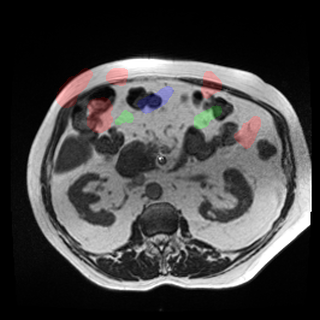
\includegraphics[width=.8\textwidth]{bilder/case7-day0-slice-0096}
    \caption{Fall 7, Tag 0 und Teilstück Nr. 96}
    \end{minipage}\hfill
    \begin{minipage}{0.45\textwidth}
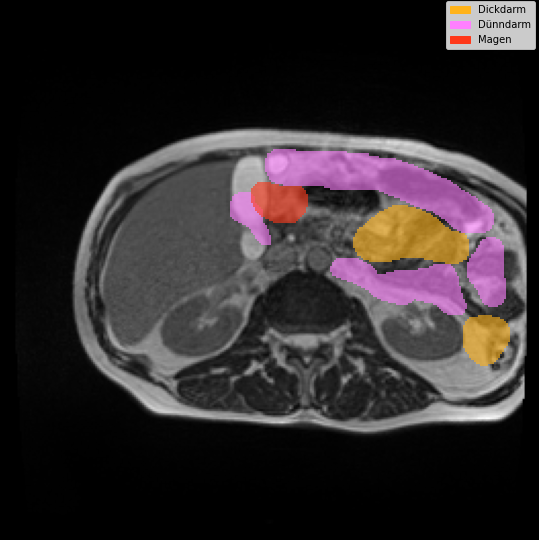
\includegraphics[width=.8\textwidth]{bilder/case81-day30-slice-0096}
    \caption{Fall 81, Tag 3 und Teilstück Nr. 96}
    \label{fig:false-seg}
    \end{minipage}
    \centering
\end{figure}

\subsection{Nacharbeit}

Bestimmte Teilstücke weisen nie eine Segmentierung auf. Dieses Wissen kann man dazu nutzen, um die Vorhersage zu bereinigen, indem man die Maske jener Teilstücke entfernt. Mithilfe dieser Methode kann man seinen Score bei Kaggle um e-3 bis e-4 verbessern. 

Im Schnitt handelt es sich um ungefähr 17 Teilstücken pro Klasse, die niemals segmentiert sind, dabei sind es immer die Stücke zu Beginn oder zum Ende eines Scans.

Ob dies jedoch good practice im Klinikalltag ist, ist fragwürdig, da diese Beobachtungen auf diesem Datensatz gemacht wurden und es wahrscheinlich ist aufgrund von z.B. einer anderen Statur, Vorerkrankungen oder anderen physikalischen Eigenschaften dies bei anderen Patienten nicht gegeben ist. 

\pagebreak

\subsection{Algorithmik}

\subsubsection{Hausdorff-Metrik} \label{ssec:hdorff}
Die Hausdorff-Metrik ist eine Methode zur Berechnung des Abstands zwischen den Segmentierungsobjekten X und Y, indem der am weitesten entfernte Punkt auf Objekt X vom nächstgelegenen Punkt auf Objekt Y berechnet wird.

\begin{equation}
d_{\mathrm{H}}(X, Y)=\max \left\{\sup _{x \in X} d(x, Y), \sup _{y \in Y} d(X, y)\right\}
\end{equation}

\subsubsection{Binäre Kreuzentropie} \label{ssec:bce}

Die Kreuzentropie ist definiert als ein Maß für die Differenz zwischen zwei Wahrscheinlichkeitsverteilungen für eine bestimmte Zufallsvariable oder eine Reihe von Ereignissen. Sie eignet sich besonders gut für Klassifizierungen auf Pixelebene, weist jedoch bei einer unausgewogenen Klassenverteilung der Daten ihre schwächen auf. \citet{Jadon_2020} 

Sie ist definiert als:
\begin{equation}
\mathcal{L}_{BCE}\left(X_{i l}, Y_{i} l\right)=\sum_{c=1}^{C} X_{i c l} \log \left(Y_{i c l}\right)
\label{eq:bce}
\end{equation}

\subsubsection{Dice-Koeffizient} \label{ssec:dc}

Der Dice-Koeffizient kann verwendet werden, um die pixelweise Übereinstimmung zwischen einer vorhergesagten Segmentierung und der entsprechenden Groundtruth zu vergleichen. Die Formel ist gegeben durch:

\begin{equation}
D S C=\frac{2|X \cap Y|}{|X|+|Y|}
\label{eq:dice}
\end{equation}

wobei X die vorhergesagte Menge von Pixeln und Y die Groundtruth ist. Der Dice-Koeffizient ist definiert als 0, wenn sowohl X als auch Y leer sind.

\subsection{Modell}

Das Projekt wurde gänzlich in Python mithilfe der TensorFlow API sowie dem
 \href{https://deepai.org/machine-learning-glossary-and-terms/relu}{Segmentation Models} \citet{Yakubovskiy:2019}
 Package aufgezogen, welches verschiedene Architekturen inklusive an- und nicht trainierte Encoder zur verfügung stellt. 
 
 Die Lossmetrik ist eine Mischung aus zu 60\% der 
binären Kreuzentropie [\ref{eq:bce}] und zu 40\% des Dice-Koeffizienten [\ref{eq:dice}]. 


\begin{equation}
\mathcal{L}\left(X_{i l},{Y_{i}} l\right)= 0.6 * \sum_{c=1}^{C} X_{i c l} \log \left({Y}_{i c l}\right)+0.4 *\left(1-\frac{2\left|X_{i l} \cap {Y_{i}} l\right|}{\left|X_{i l}\right|+\left|{Y_{i}} l\right|}\right)
\label{eq:loss}
\end{equation}

Diese Kombination eignet sich laut \citet{Jadon_2020} et al. besonders gut, um einen höheren Dice Score zu erzielen. Außerdem ermöglicht sie dem Modell, sich auf mehrere Klassen zu konzentrieren, so ist das Modell in der Lage das Klassenungleichgewicht zu berücksichtigen. 

 Trainiert wurde mit dem
\href{https://optimization.cbe.cornell.edu/index.php?title=Adam}{Adam Optimizer}
 und einer initialen Lernrate von von 5e-4, die sich um den Faktor e-1 verringert, wenn die Validierungsmetrik nach fünf Epochen keine Verbesserung vorwies.

Die Daten wurden in 5 Folds aufgeteilt und anhand des Falles getrennt. Hierbei wurde beachtet, dass die einzelnen Folds die Verteilung der Klassen beibehielten.
Die Daten wurden mithilfe von der 
\href{https://scikit-learn.org/stable/modules/generated/sklearn.model_selection.StratifiedGroupKFold.html}{StratifiedGroupKFold} Methode von Sklearn aufgeteilt nach mit einem  Zufalls-Seed von 42.

Folgende Parameter konnten über die Kommandozeile konfiguriert werden:
\begin{itemize}
\item Encoder
\item Eingabegröße
\item Batchsize
\item Epochen
\item Validierungsfold
\end{itemize}

Außerdem konnten folgende Features angewendet werden:
\begin{itemize}
\item 2.5 dimensionale Trainigsdaten \ref{ssec:semi3d-data}
\item Intelligentes Zuschneiden \ref{ssec:intellicrop}
\item Bereinigen der Trainingsdaten \ref{ssec:clean-data}
\end{itemize}

\subsection{Experimente}

\subsubsection{Ablauf}

Das Training erfolgte gänzlich auf dem \href{https://wiki.hhu.de/display/HPC/Abschlussarbeiten+im+HPC}{Hochleistungs-Rechencluster} des ZIMs. Zum einsatz kamen verschiedene Grafikkarten: RTX 8000, RTX 6000, GTX 1080ti sowie der Nvidia DGB A100, je nach Verfügbarkeit und Anspruch der Modelle. 

Es wurden folgende Module des HPC's verwendet: 
\begin{itemize}
\item Python/3.8.3
\item gcc/10.2.0
\item CUDA/11.2.2
\item bazel/0.28.0
\item cuDNN/8.1.1
\end{itemize}

Mithilfe eines \href{https://github.com/vitoleonardo/HealthyOrganTracker/blob/main/jobscript/job}{Skripts} wurden die jeweiligen Konfigurationen über die Kommandozeile übergeben. 

Nach abgeschlossenem Training wurden Vorhersagungen auf dem Validierungsfold getroffen, dabei wurde pro Teilstück und Klasse der Dice-Koeffizient berechnet um im Anschluss die besten und schlechtesten Fälle zu evaluieren.

Dazu wurde aufgrund des hohen Rechenaufwands ebenfalls ein \href{https://github.com/vitoleonardo/HealthyOrganTracker/blob/673a743c99af3771f88289eca6db33ab7d1bfe48/hpc_train_files/util/getperformance.py}{Skript} erstellt, welches vom Hochleistungs-Rechencluster ausgeführt worden werden konnte. 

\subsubsection{Baseline}

Zunächst wurde eine Baseline mit folgenden Standardkonfigurationen geschaffen, um einen Encoder ausfindig zu machen:

\begin{table}[H]
\centering
\resizebox{\textwidth}{!}{\begin{tabular}{l|c|c|c|c|c}
Input & Batchsize & Epochen & Datenbereinigung & 2.5 Daten & Intelligentes Zuschneiden\\\hline
256x256x1 & 16 & 50 & Falsch & Falsch & Falsch\\
\end{tabular}}
\caption{\label{tab:widgets}Baseline Einstellungen}
\end{table}

Basierend darauf wurden 12 Modelle trainiert, wessen Encoder auf
\href{https://www.image-net.org/}{ImageNet} angelernt wurden:

\begin{table}[H]
\resizebox{\textwidth}{!}{\begin{tabular}{l|c|c|c|c|c|c|c}
       Encoder & Beste Epoche &   Loss & Val. loss &   Dice & Val. Dice &    IoU & Val. IoU \\\hline
efficientnetb2 &           26 & 0.0364 &   \textbf{ 0.1198} & 0.9156 &   \textbf{ 0.7307} & 0.8969 &   0.8163 \\
efficientnetb6 &           39 & \textbf{0.0321} &    0.1222 & \textbf{0.9256} &    0.7227 & \textbf{0.9220} &   \textbf{0.8218} \\
efficientnetb5 &           25 & 0.0379 &    0.1232 & 0.9123 &    0.7191 & 0.8866 &   0.8167 \\
   densenet201 &           32 & 0.0390 &    0.1239 & 0.9097 &    0.7191 & 0.8927 &   0.8091 \\
efficientnetb7 &           18 & 0.0408 &    0.1245 & 0.9056 &    0.7143 & 0.8988 &   0.8171 \\
efficientnetb1 &           27 & 0.0369 &    0.1263 & 0.9147 &    0.7123 & 0.8907 &   0.8082 \\
efficientnetb4 &           22 & 0.0382 &    0.1278 & 0.9117 &    0.7081 & 0.9011 &   0.8158 \\
   inceptionv3 &           22 & 0.0420 &    0.1352 & 0.9028 &    0.6885 & 0.8652 &   0.8036 \\
efficientnetb0 &           26 & 0.0375 &    0.1444 & 0.9131 &    0.6678 & 0.9025 &   0.7932 \\
   densenet121 &           30 & 0.0425 &    0.1699 & 0.9017 &    0.6019 & 0.8758 &   0.7824 \\
efficientnetb3 &           22 & 0.0387 &    0.1753 & 0.9103 &    0.5887 & 0.8770 &   0.7823 \\
      resnet50 &           19 & 0.0415 &    0.1795 & 0.9040 &    0.5797 & 0.8675 &   0.7600 \\
\end{tabular}}
\caption{\label{tab:baselines}Baseline Performances nach Validation loss absteigend sortiert.}
\end{table}

EfficientNet-b2 führt die Tabelle an mit einem Val. loss von 0.1198 und einem Val. Dice-Koeffizienten von 0.7307. Ebenfalls zu beobachten ist eine starke Korrelation zwischen [\ref{eq:loss}] und [\ref{eq:dice}], dies bestärkt die Aussage von \citet{Jadon_2020} et al., dass sich [\ref{eq:loss}] gut dazu eignet, um einen höheren Dice-Koeffizienten zu erzielen.

\begin{figure}[H]
	\begin{center}
		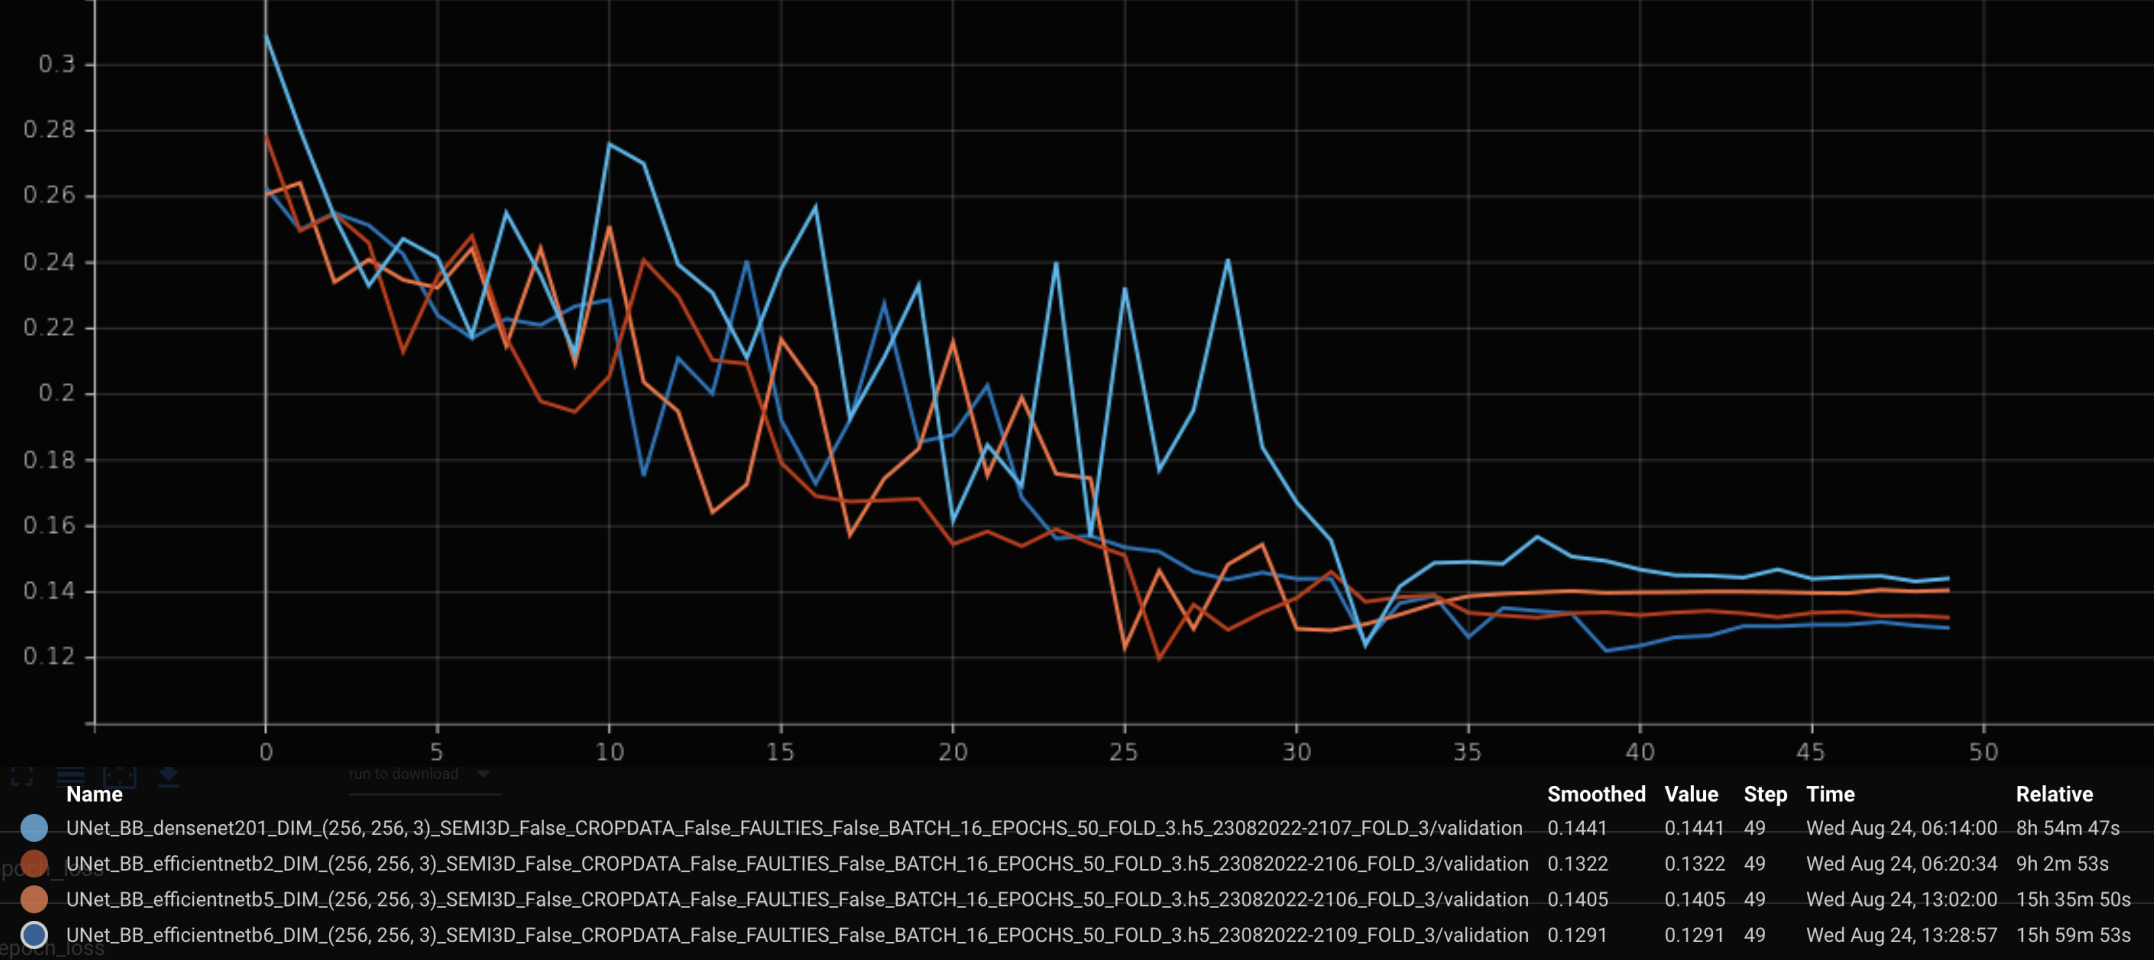
\includegraphics[width=400pt]{LaTex/bilder/256_val_loss.png}
		\caption{Entwicklung der Validation Loss-Metrik der Top 4}\label{Fig:256_train}
	\end{center}
\end{figure}

Wie in \autoref{Fig:256_train} zu sehen konvergieren die Modelle ab Epoche 35, eine Verbesserung der Loss-Metrik ist demnach nicht weiter absehbar. In Epoche 50 führt b6, gefolgt von b2, b5 und densenet201. 

Somit bildet das Modell mit denm Encodern EfficientNet-b2 die Baseline dieser Arbeit.

\subsection{Batchgröße}

Experimente mit größeren Batches haben, falls das Training überhaupt erfolgte, stets zu einer Verschlechterung der Werte geführt und werden hier deswegen nicht weiter behandelt.

\pagebreak

\section{Evaluation}\raggedbottom

Die Auswertung erfolgte auf 2 Arten:
\begin{enumerate}
\item Lokal anhand der Werte des Dice-Koeffizienten vom Validierungsset \ref{ssec:dc}
\item Online anhand der Evaluationsmetrik der Kaggle-Challenge \ref{ssec:kaggle}
\end{enumerate}

\subsection{EfficientNet-b2}

\begin{table}[H]
\centering
\resizebox{\textwidth}{!}{\begin{tabular}{c|c|c|c|c|c|c|c|c}
Beste Epoche &   Loss &   Dice  & Dickdarm & Dünndarm &  Magen &  2.5D &  Crop & Bereinigt  \\\hline
          36 &\textbf{ 0.0326 }& \textbf{0.9244} &  0.9282 & 0.9042 &\textbf{ 0.9385 }&  True & False &      True  \\
          29 & 0.0340 & 0.9214  &   0.9261 &   0.8995 & 0.9352 & False &  True &      True  \\
          31 & 0.0336 & 0.9226  &   0.9266 &   0.9019 & 0.9377 &  True &  True &      True  \\
          42 & 0.0315 & 0.9274  &   \textbf{0.9322}  &   \textbf{0.9088} & 0.9380 & False &  True &     False  \\
          32 & 0.0327 & 0.9241  &   0.9283 &   0.9038 & 0.9380 &  True & False &     False  \\
          26 & 0.0353 & 0.9181  &   0.9211 &   0.8957 & 0.9325 & False & False &      True  \\
          34 & 0.0322 & 0.9257  &   0.9304 &   0.9057 & 0.9374 &  True &  True &     False  \\
\end{tabular}}
\caption{\label{tab:efb2-train} Performance von EfficientNet-b2 auf dem Trainingsdatensatz.}
\end{table}


\begin{table}[H]
\centering
\resizebox{\textwidth}{!}{\begin{tabular}{c|c|c|c|c|c|c|c|c|c}
Index & Beste Epoche & Loss      &  Dice     &  Dickdarm     & Dünndarm      & Magen       &  2.5D &  Crop & Bereinigt \\\hline
 1    &     36 &    0.0919 &    0.7983 &        0.8271 &        0.7709 &     0.8412  &  True & False &      True\\
 2    &     29 &    0.0950 &    0.7904 &        0.8292 &        \textbf{0.7760} &     0.8505  & False &  True &      True\\
 3    &     31 &    0.0954 &    0.7873 &        \textbf{0.8365} &        0.7724 &     \textbf{0.8527 } &  True &  True &      True\\
 4    &     42 &    0.0985 &    0.7850 &        0.8091 &        0.7709 &     0.8391  & False &  True &     False\\
 5    &     32 &    0.1037 &    0.7691 &        0.8140 &        0.7753 &     0.8161  &  True & False &     False\\
 6    &     26 &    0.1071 &    0.7587 &        0.8106 &        0.7423 &     0.8242  & False & False &      True\\
 7    &     34 &    0.1096 &    0.7530 &        0.8056 &        0.7537 &     0.7904  &  True &  True &     False\\
\end{tabular}}
\caption{\label{tab:efb2-val} Performance von EfficientNet-b2 auf dem Validierungsdatensatz.}
\end{table}

Das Verwenden von Features liefert in jedem Fall eine Steigerung des Dice-Koeffizienten (+ 0.223 bis + 0.676). Am schlechtesten war die Kombination aus 2.5 dimensionalen und zugeschnittenen Daten, am besten die aus 2.5 dimensionalen und bereinigten Daten. Das Zusammenspiel aller Erweiterungen liegt auf dem dritten Platz, jedoch nur mit einem kleinen Abstand von 0.11 zum ersten Platz. 

Gemessen an den einzelnen Klassen liefert das Modell welches über alle Erweiterungen verfügt die besten Ergebnisse, die Punktzahl für Dickdarm und Magen ist hier am höchsten. 

\subsubsection{Stärken}

Zum Auswerten der Stärken und Schwächen der verschiedenen Erweiterungen sowie deren Kombination wurde folgendes Verfahren angewendet:

\begin{enumerate}
\item Lade die Ergebnisse der Vorhersage von jedem Modell.
\item Nehme die 10 Teilstücke, die den geringsten $
\varnothing
$ Dice-Koeffizienten vorweisen. ($\varnothing$ Score der einzelnen Klassen) 
\item  Gruppiere nach Häufigkeit des Vorkommens.
\item Analysiere Teilstücke, angefangen mit jenem welches am häufigsten vertreten ist.
\end{enumerate}

\begin{itemize}
\item Fall 123 Tag 20 Teilstück 73
\end{itemize}

\begin{figure}[H]
	\begin{center}
		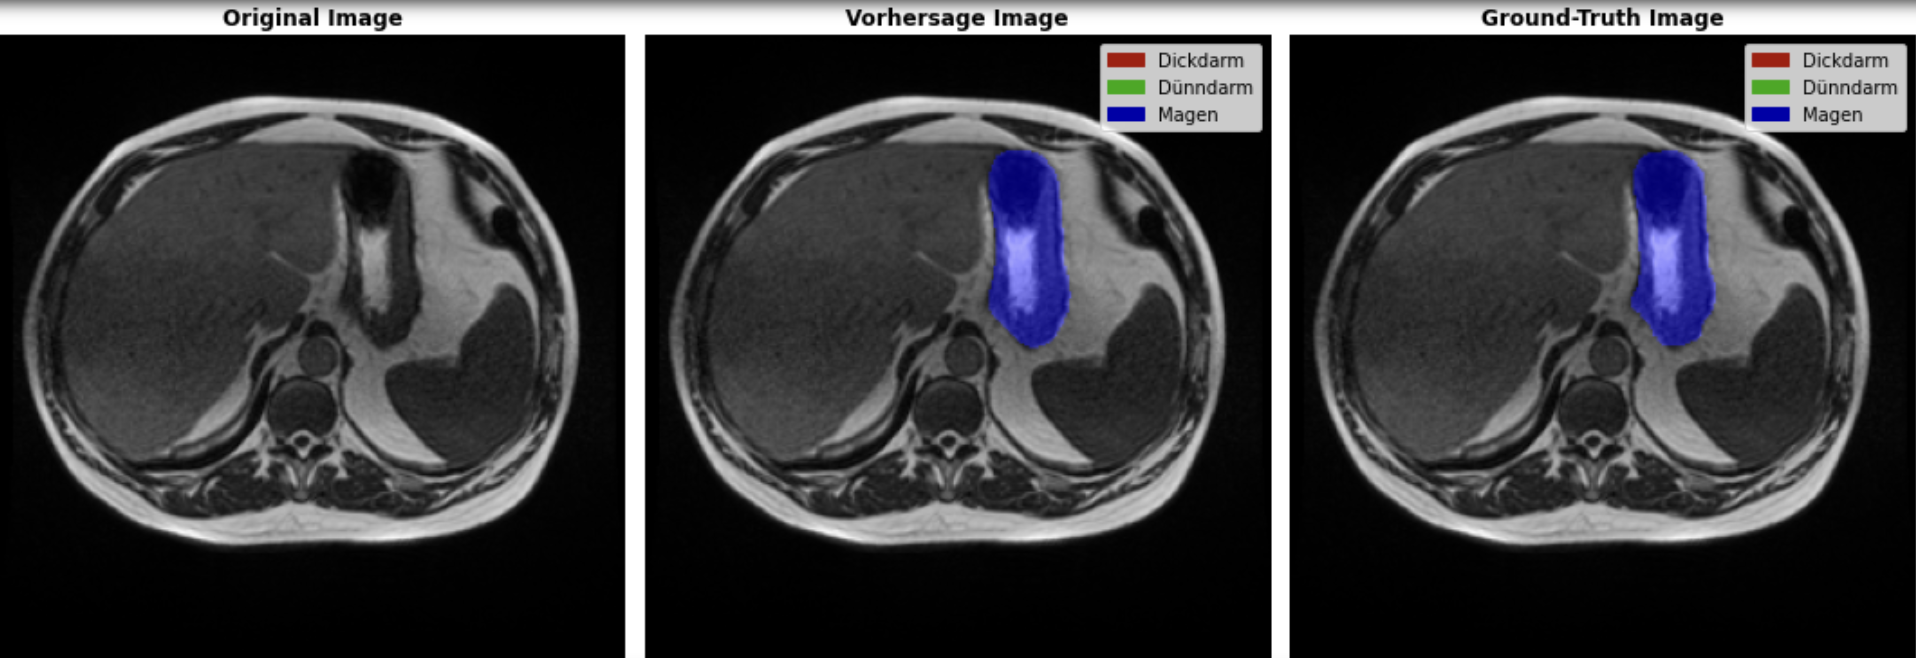
\includegraphics[width=400pt]{LaTex/bilder/case123_day20_slice_0073.png}
		\caption{ Teilstück mit dem höchsten Dice-Koeffizienten }\label{Fig:7vs1}
	\end{center}
\end{figure}

Dieses Teilstück wurde von allen Modellen mit einem Score von über 0.97 segmentiert. 

\begin{itemize}
\item Fall 33 Tag 21 Teilstück 86
\end{itemize}

\begin{figure}[H]
	\begin{center}
		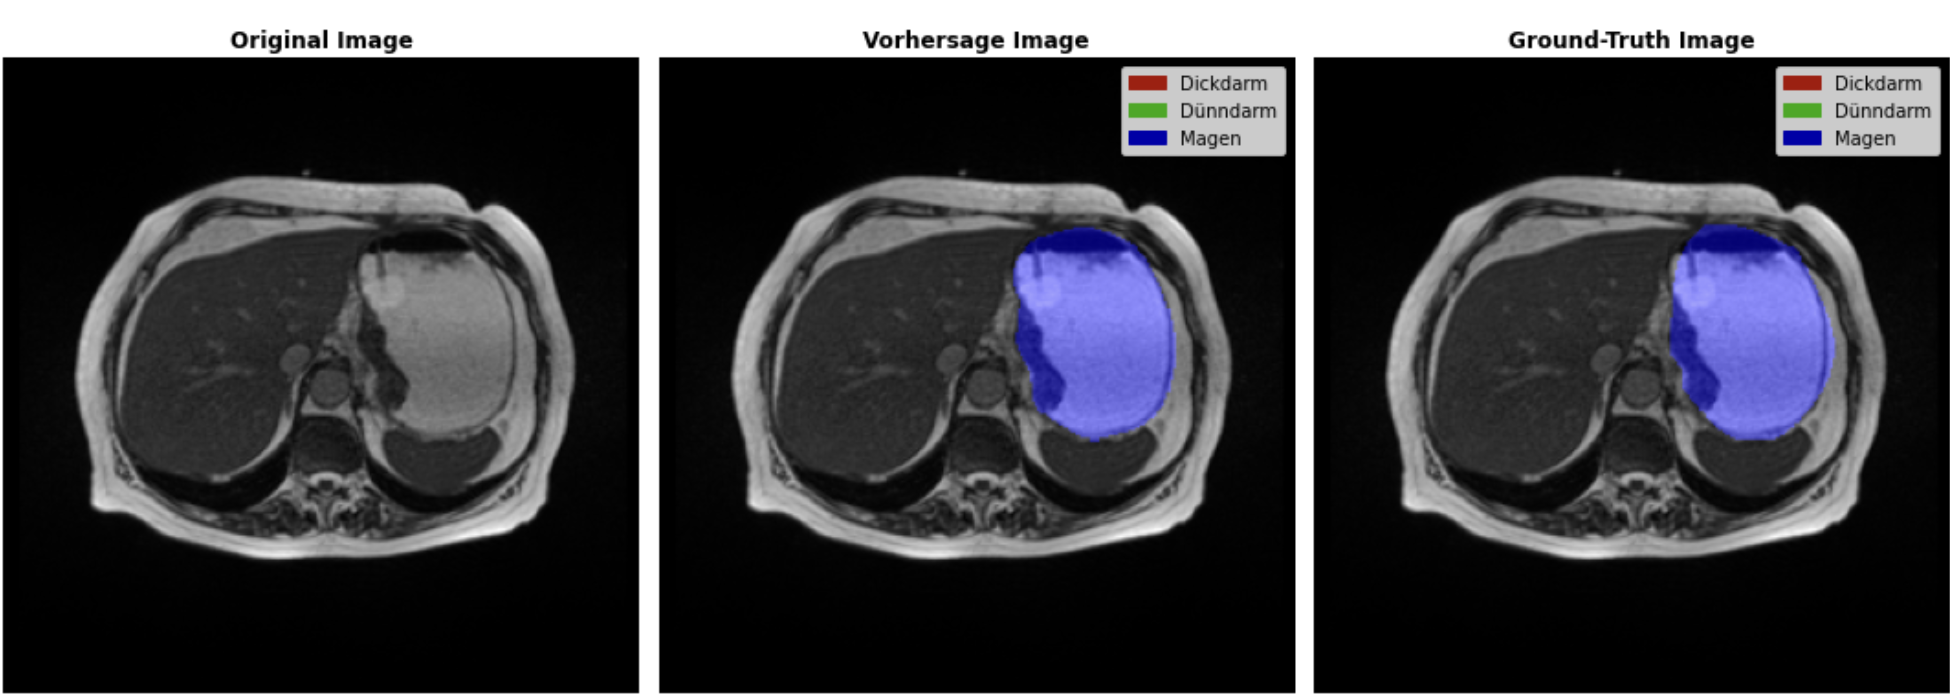
\includegraphics[width=400pt]{LaTex/bilder/case33_day21_slice_0086.png}
		\caption{ Akkurate Segmentierung des Magens }\label{Fig:7vs1}
	\end{center}
\end{figure}

\pagebreak

\begin{itemize}
\item Fall 36 Tag 10 Teilstück 60
\end{itemize}

\begin{figure}[H]
	\begin{center}
		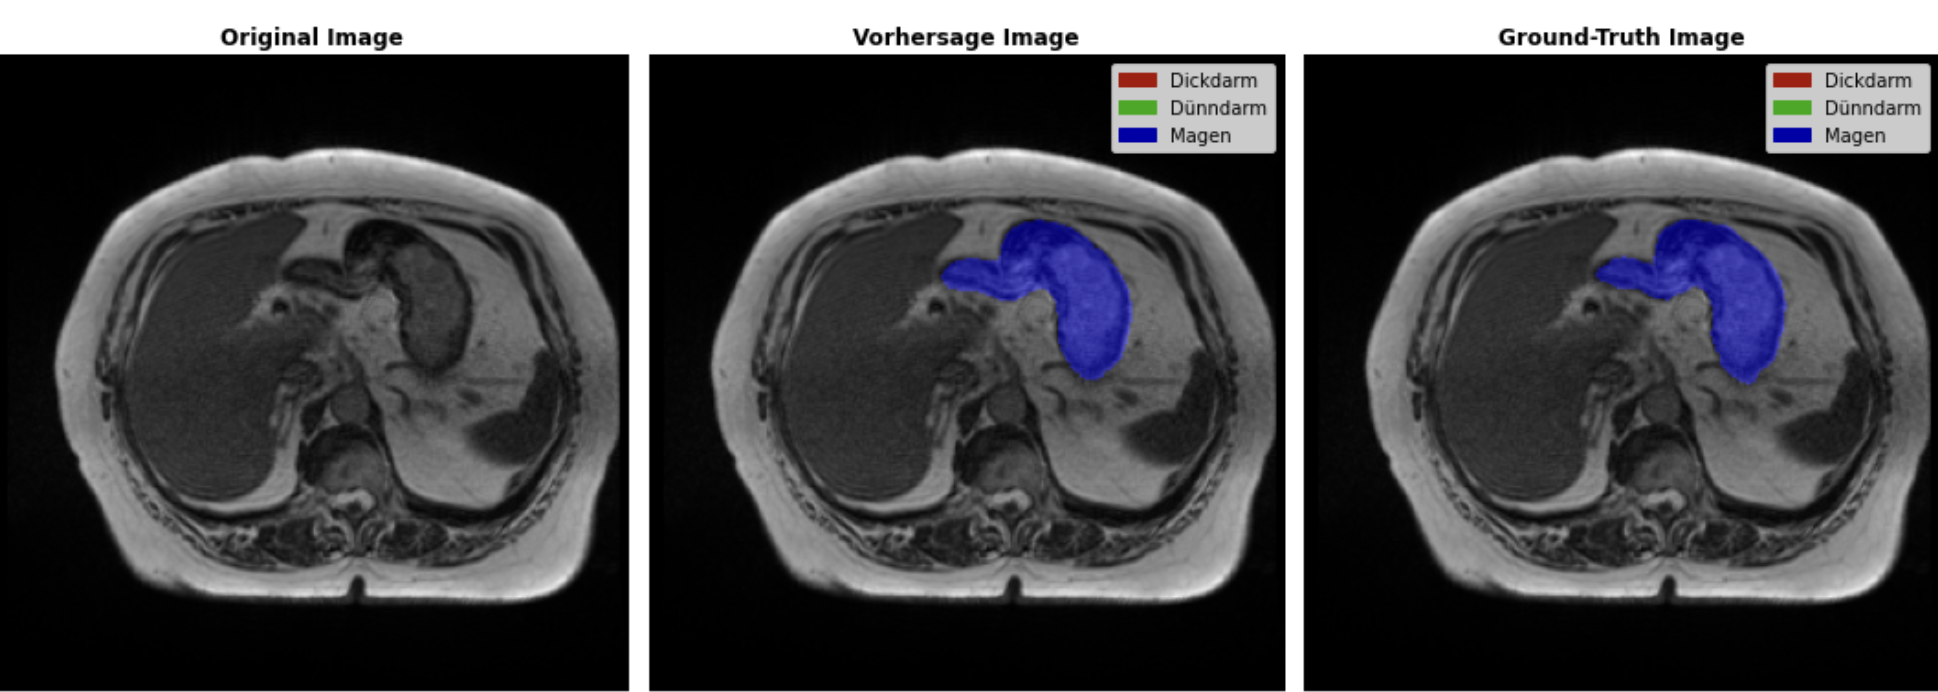
\includegraphics[width=400pt]{LaTex/bilder/case36_day10_slice_0060.png}
		\caption{  }\label{Fig:7vs1}
	\end{center}
\end{figure}

Jedes Modell konnte diese Teilstücke mit einer Genauigkeit von über 0.96 gemessen am Dice-Koeffizienten segmentieren.

Die Beobachtung setzt sich genauso weiter fort, es sind immer Teilstücke auf denen der Magen sehr gut erkannt worden ist. Dadurch dass der Magen im Gegensatz zu den anderen beiden Organen seine Position im Körper relativ konstant beibehält sind die Ergebnisse stimmig.

Nun zu den Teilstücken, die mindestens 2 Organe abbilden:

\begin{itemize}
\item Fall 156 Tag 11 Teilstück 110
\end{itemize}

\begin{figure}[H]
	\begin{center}
		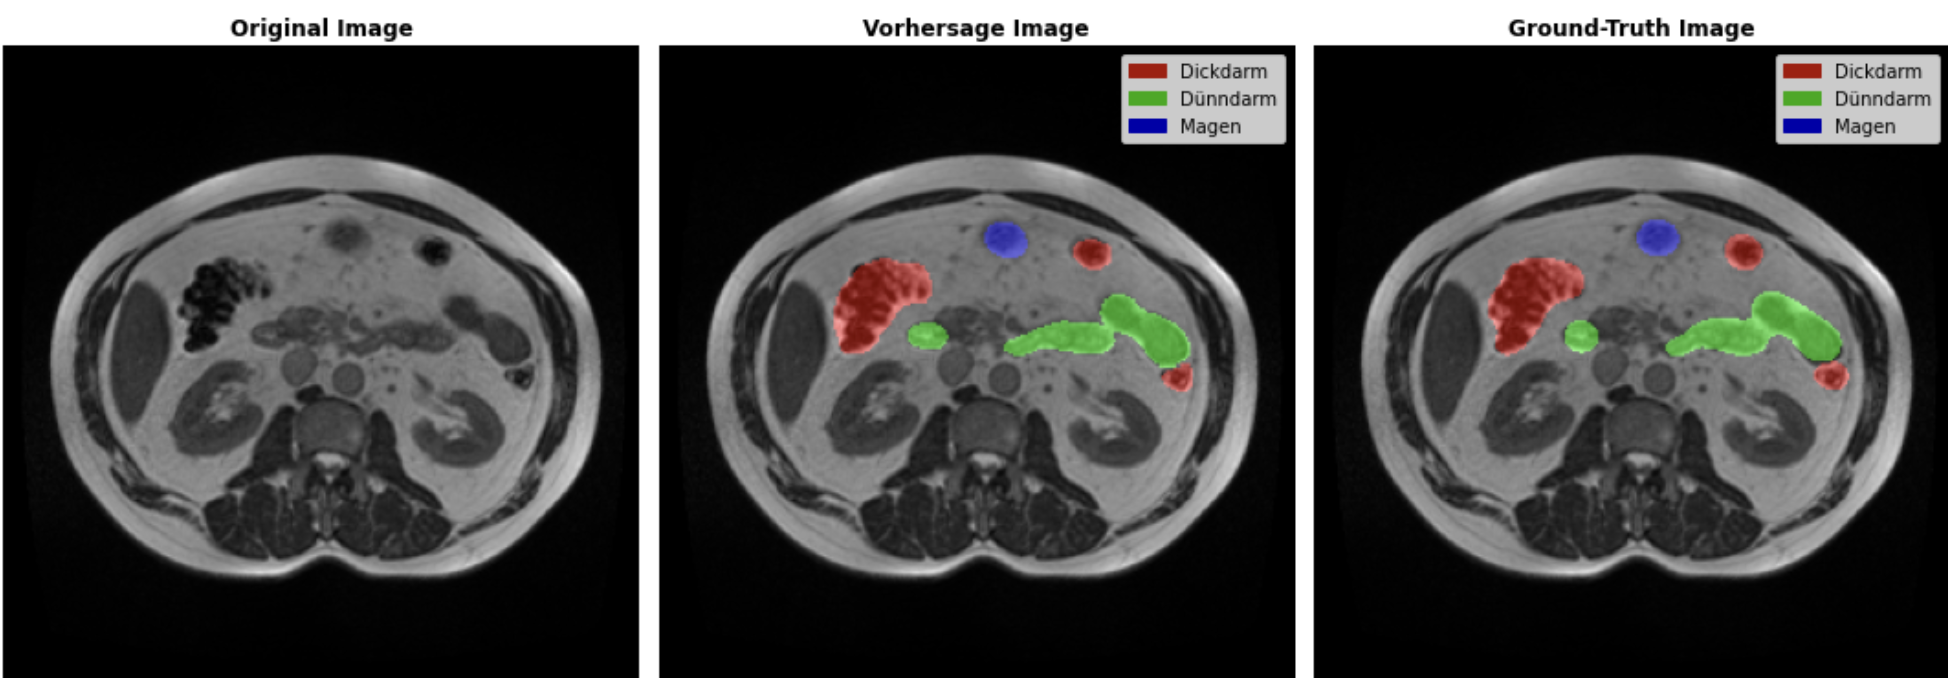
\includegraphics[width=400pt]{LaTex/bilder/case156_day11_slice_0110.png}
		\caption{  }\label{Fig:7vs1}
	\end{center}
\end{figure}

Die Baseline weist hierbei den geringsten Score von 0.81 auf, Nr 6 und 1 erzielen hier über 0.92.

\pagebreak

\begin{itemize}
\item Fall 41 Tag 32 Teilstück 106
\end{itemize}

\begin{figure}[H]
	\begin{center}
		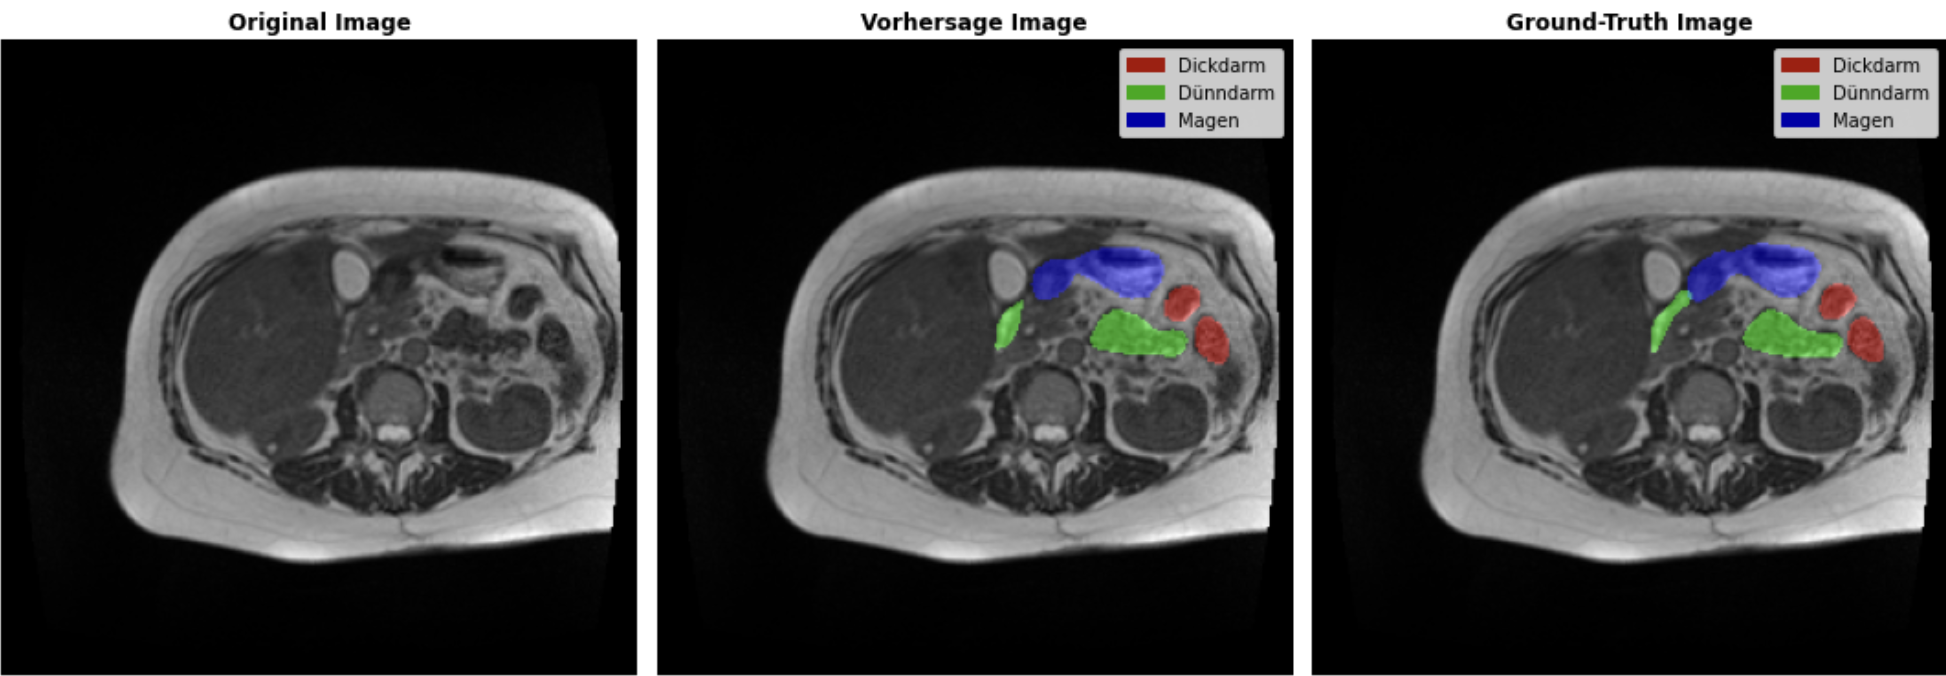
\includegraphics[width=400pt]{LaTex/bilder/case41_day32_slice_0106.png}
		\caption{ Vorhersage von Model Nr 2 mit einem Score von 0.92 }\label{Fig:analysis-clean-data}
	\end{center}
\end{figure}

Hierbei macht sich das entfernen der schlecht segmentierten Trainingsbilder deutlich: Modelle ohne jenes Feature haben einen Score von 0.56 - 0.86, wohingegen die restlichen auf über 0.91 kommen. 

\begin{itemize}
\item Fall 18 Tag 19 Teilstück 79
\end{itemize}

\begin{figure}[H]
	\begin{center}
		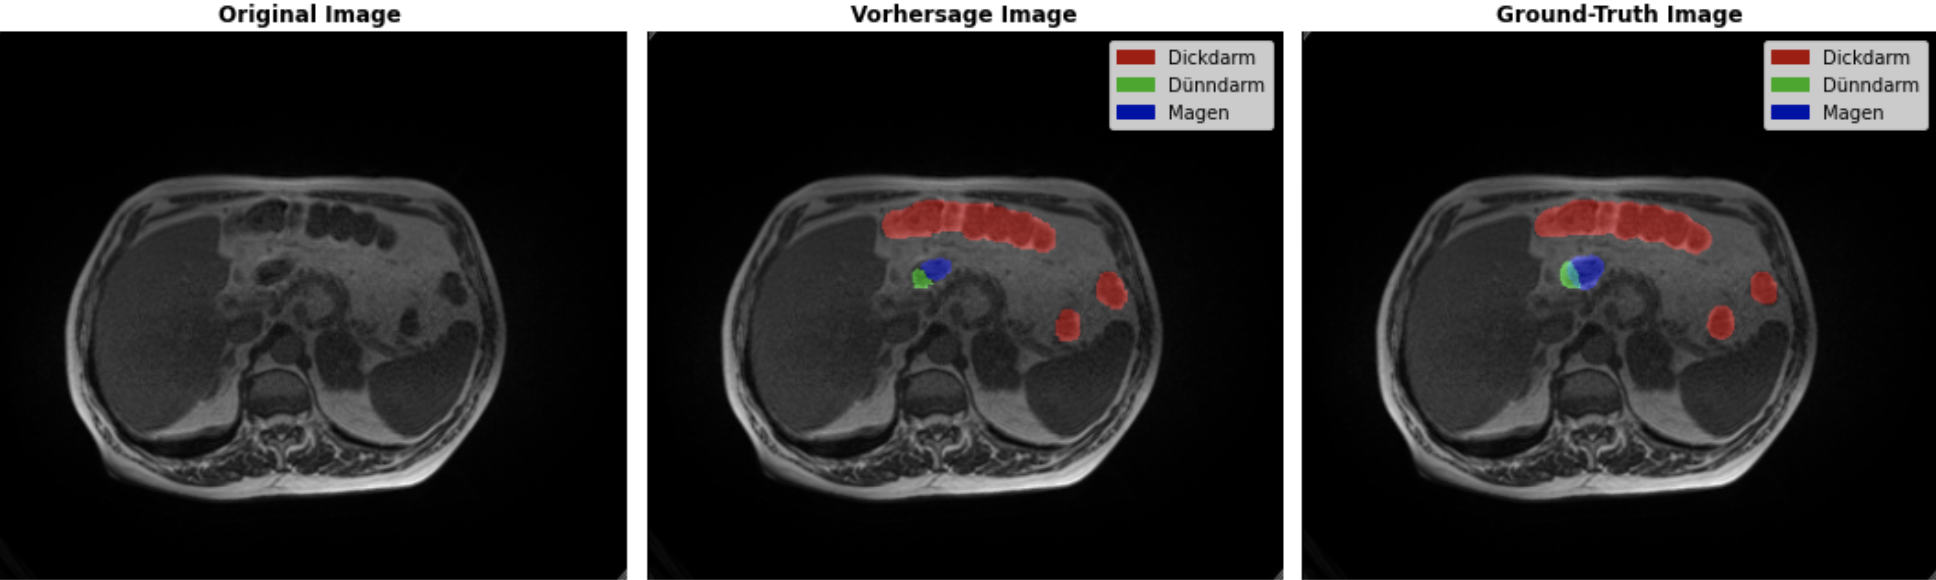
\includegraphics[width=400pt]{LaTex/bilder/case18_day19_slice_0079.png}
		\caption{ Vorhersage von Model Nr. 7 mit einem Score von 0.73 }\label{Fig:trade-off}
	\end{center}
\end{figure}

Interessanterweise führt hier das Modell, welches mit allen Features bis auf die Bereinigung der Daten trainiert wurde mit einem Abstand von 0.06 zu Modell Nr 1., welches mit allen Features trainiert wurde. Modell 1 hatte hier Schwierigkeiten den Dünndarm neben dem Magen zu erkennen. 

\pagebreak

\subsubsection{Schwächen}

\begin{itemize}
\item  Fall 88 Tag 0 Teilstück 121 und 122
\end{itemize}

\begin{figure}[H]
	\begin{center}
		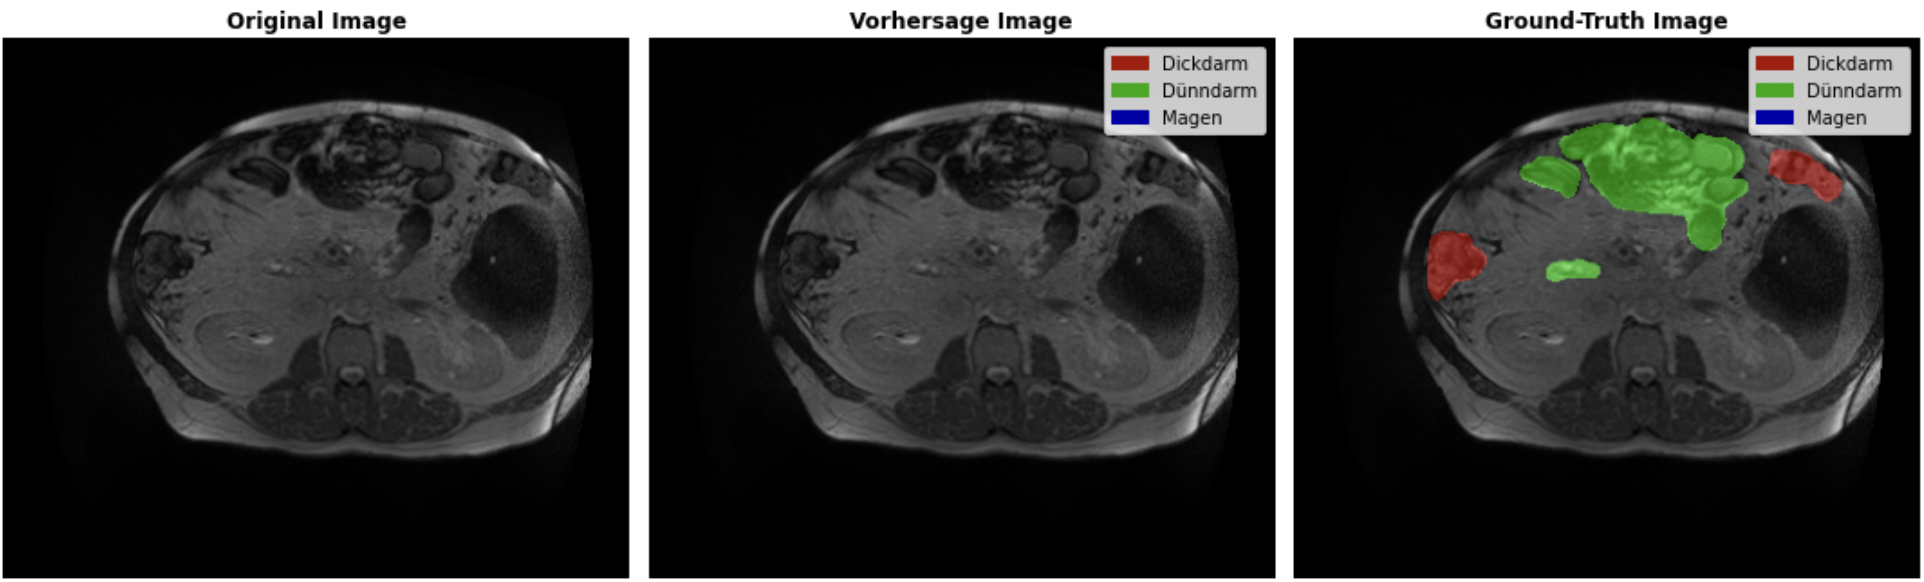
\includegraphics[width=400pt]{LaTex/bilder/case88_day0_slice_0121.png}
		\caption{ Nicht-segmentiertes Teilstück 121 }\label{Fig:7vs1}
	\end{center}
\end{figure}

Alle obigen Modelle haben für dieses Teilstück keine Segmentierung vorhergesagt obwohl dort der Dick- und Dünndarm zu sehen ist. 

\begin{itemize}
\item  Fall 88 Tag 0 Teilstück 120
\end{itemize}
\begin{figure}[H]
	\begin{center}
		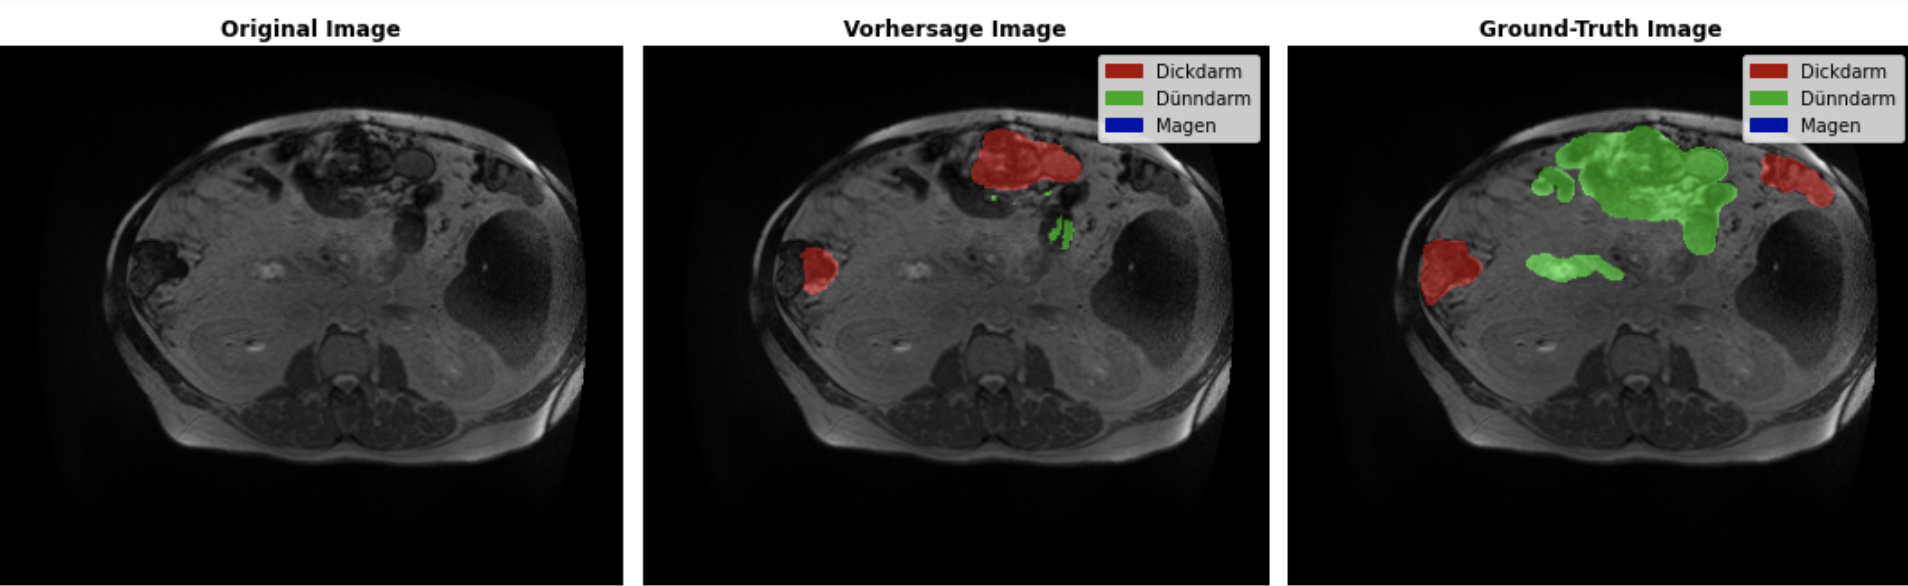
\includegraphics[width=400pt]{LaTex/bilder/case88_day0_slice_0120_no2.png}
		\caption{ Einzige Vorhersage von Modell Nr. 2 }\label{Fig:7vs1}
	\end{center}
\end{figure}
Hier konnte einzig das zweite Modell etwas erkennen mit einem Score von 0.13

\begin{itemize}
\item Fall 88 Tag 0 Teilstück 119
\end{itemize}
\begin{figure}[H]
	\begin{center}
		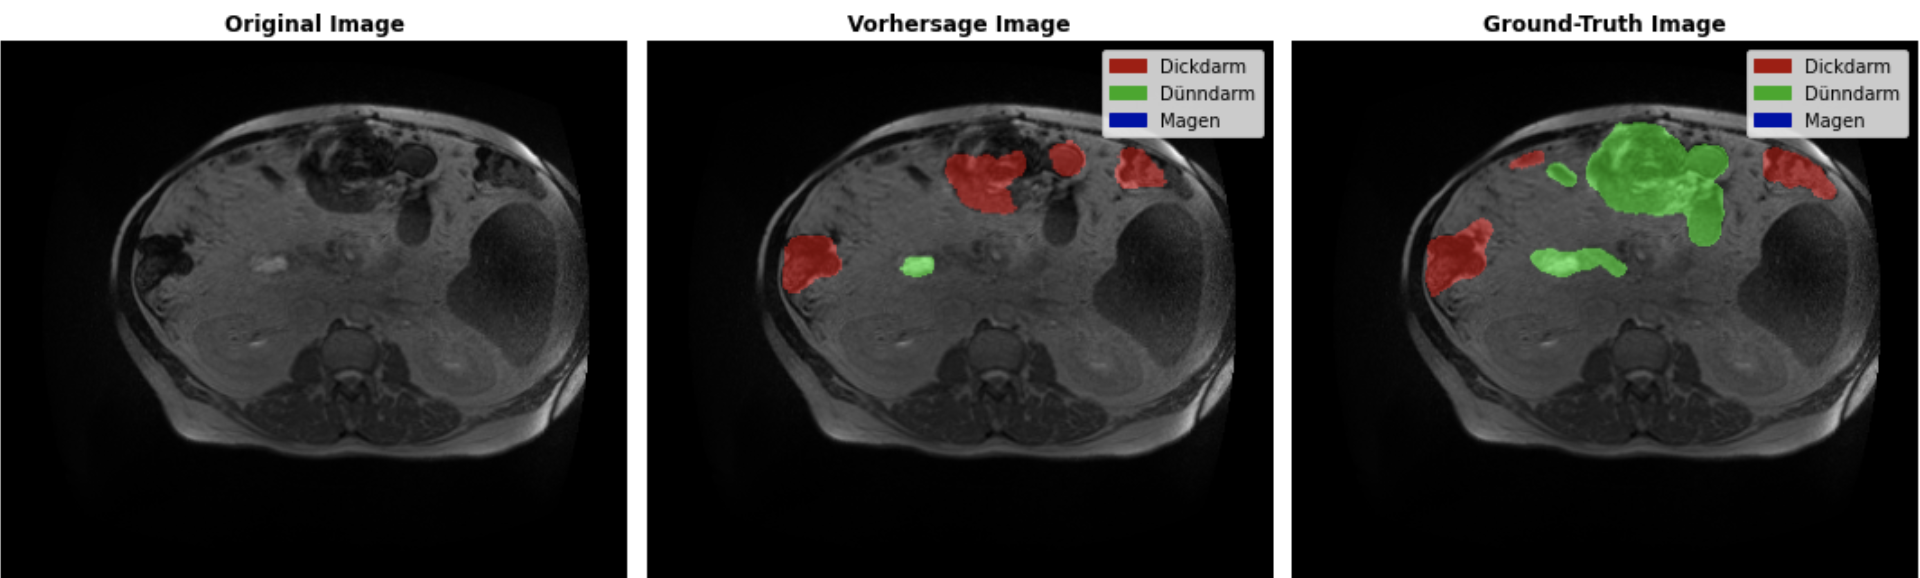
\includegraphics[width=400pt]{LaTex/bilder/case88_day0_slice_0119_no7.png}
		\caption{ Höchster Dice-Koeffizient von Modell Nr. 7 }\label{Fig:7vs1}
	\end{center}
\end{figure}
Die Baseline, Nr. 2 und 7 erkannten Organe mit einem Score von 0.25 +- 0.6. An erster Stelle ist die Nr. 7 mit 0.3 gefolgt von der Baseline mit 0.26.

\begin{itemize}
\item  Fall 34 Tag 16 Teilstück 72
\end{itemize}
\begin{figure}[H]
	\begin{center}
		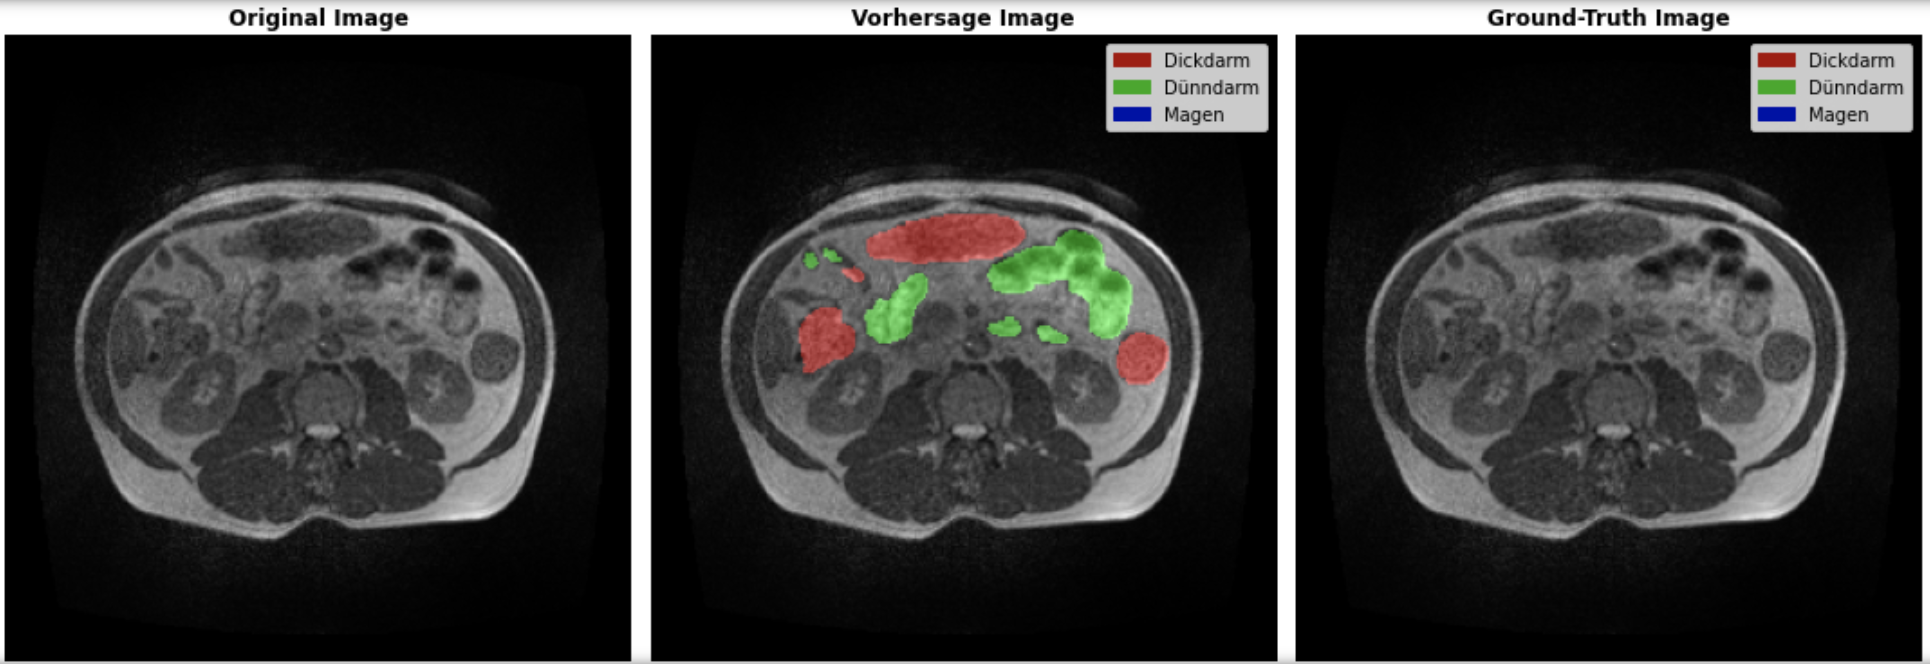
\includegraphics[width=400pt]{LaTex/bilder/case34_day16_slice_0072_no1.png}
		\caption{ False-Positive Vorhersage von Nr. 1 }\label{Fig:7vs1}
	\end{center}
\end{figure}

In diesem Beispiel lieferten alle Modelle außer die Baseline und Nr. 5 eine False-Positive Vorhersage.
\pagebreak

\begin{itemize}
\item Fall 40 Tag 17 Teilstück 122 und 123
\end{itemize}
\begin{figure}[H]
	\begin{center}
		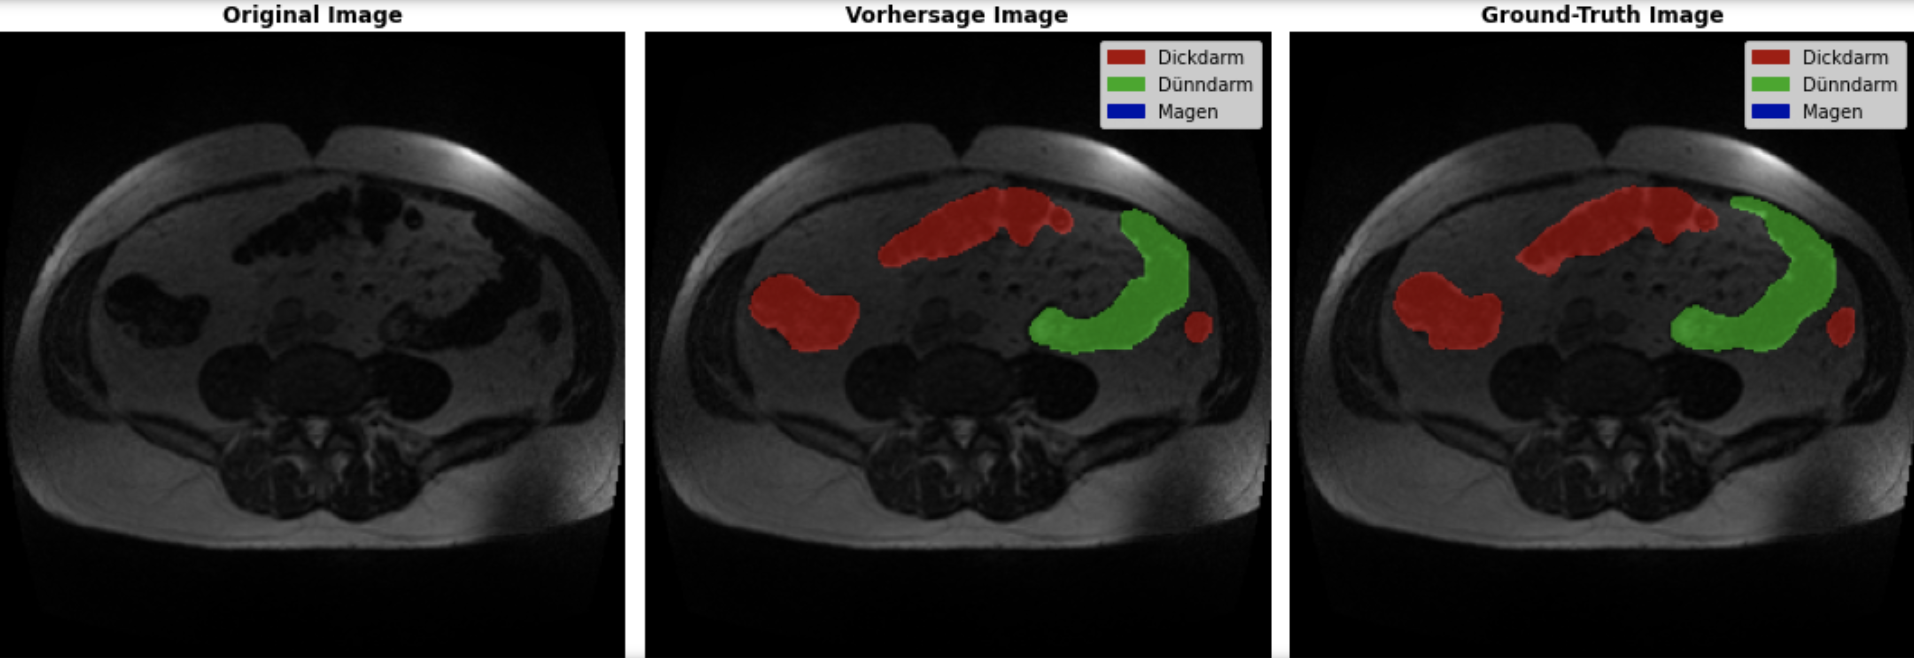
\includegraphics[width=400pt]{LaTex/bilder/case40_day17_slice_0122_no1.png}
		\caption{ Vorhersage von Modell Nr. 1 (0.935) }\label{Fig:analysis-clean-data-weak}
	\end{center}
\end{figure}
Modell Nr. 1, 2, 3, und 6 erkannten hier mit einem Score von über 0.9 eine Segmentierung, der Rest lieferte ein False-Negative Vorhersage. Auch hier sind klar die Auswirkungen von schlecht annotierten Daten zu erkennen: alle Modelle die mit diesen Daten trainiert wurden erkannten hier nichts.

\begin{itemize}
\item Fall 40 Tag 17 Teilstück 121
\end{itemize}

\begin{figure}[H]
	\begin{center}
		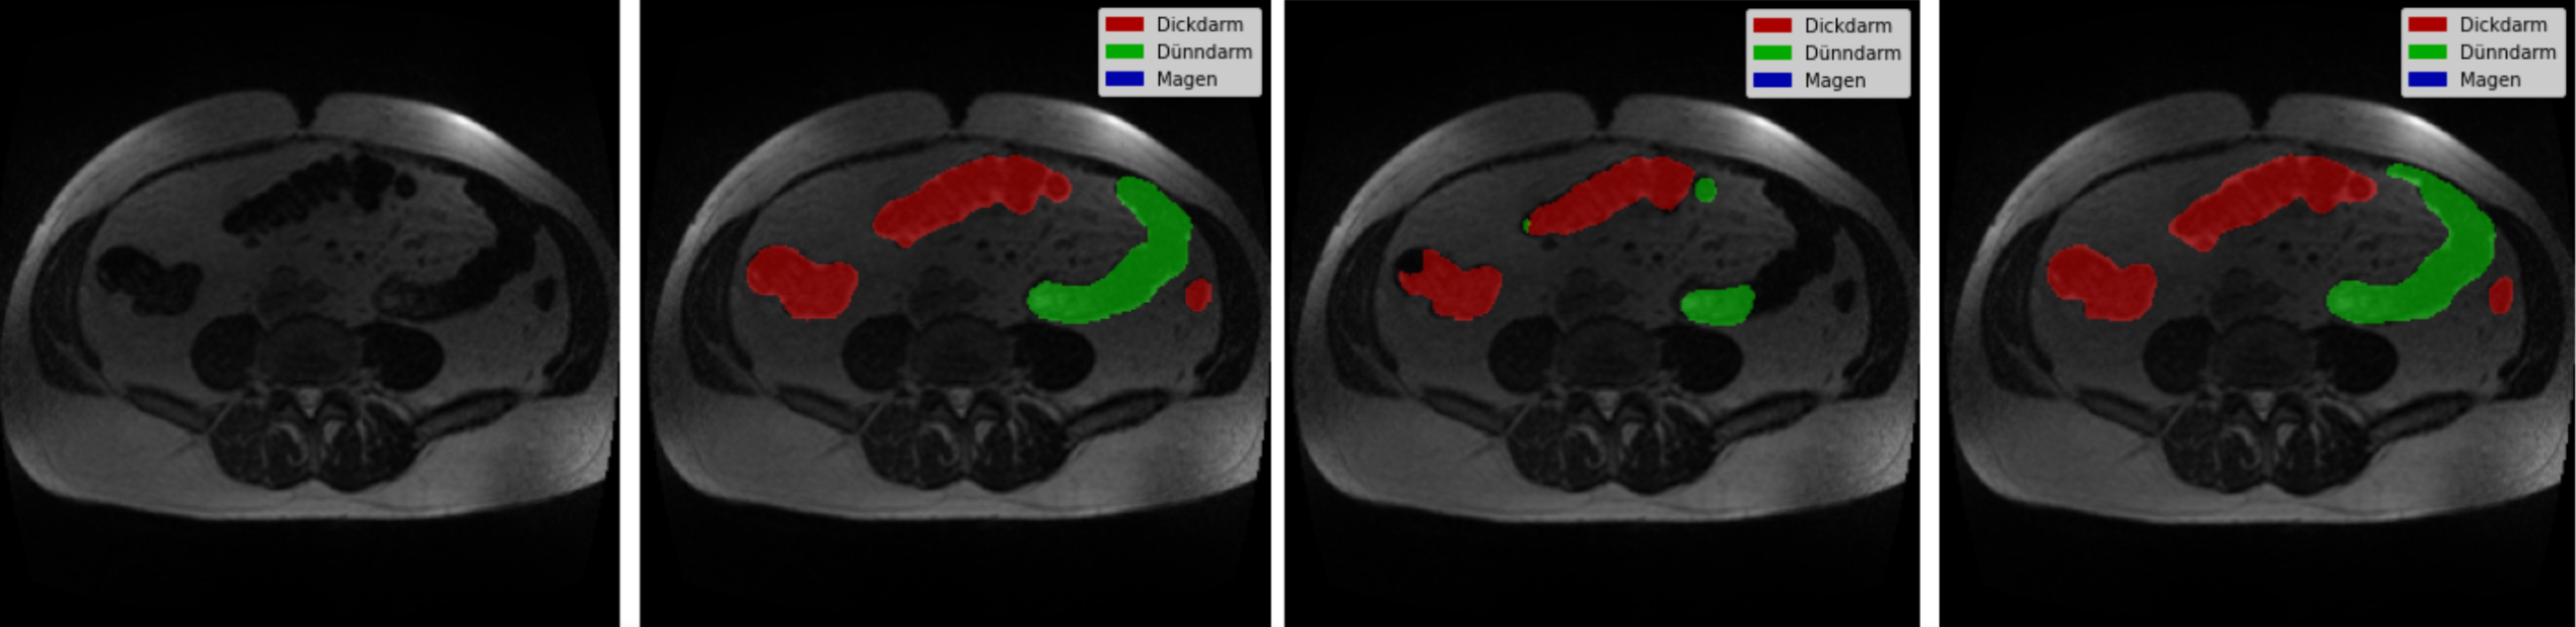
\includegraphics[width=400pt]{LaTex/bilder/case40_day17_slice122_7vs1.png}
		\caption{Links Original, gefolgt von Nr. 1 (0.935), Nr 7 (0.58) und der tatsächlichen Maske. }\label{Fig:7vs1}
	\end{center}
\end{figure}

Die Baseline, Nr. 4 und 5 lieferten hier ein False-Negative. Die restlichen Modelle bis auf Nr. 7 wiesen einen Score von über 0.92 auf. Auch hier weisen alle Modelle, dessen Daten nicht bereinigt wurden die schlechtesten Ergebnisse. 

\begin{table}[H]
\centering
\begin{tabular}{c|c|c|c}
Index & False-Negative & False-Positive & Dice-Koeffizienten  \\\hline
 1    &     4         &    2       &  0.9 u. 0.92   \\
 2    &     2         &    2       & 0.13 u. 0.19 u. 0.9 u. 0.92    \\
 3    &     4         &    2       & 0.92 u. 0.92   \\
 4    &     6         &    2       & 0    \\
 5    &     6         &    0       & 1 u. 1    \\
 6    &     4         &    2       & 0.9 u. 0.92 \\
 7    &     4         &    2       & 0.3 u. 0.56 \\
 Baseline&  5        &    0       & 0.26 u. 1 u. 1\\

\end{tabular}
\caption{\label{tab:efb2-val} Performance von EfficientNet-b2 auf dem Validierungsdatensatz.}
\end{table}

\subsection{Gegenüberstellung der Features}

\subsubsection{Entfernen falsch annotierter Daten}

Das Entfernen von falsch annotierten Datensätzen hilft den Modellen für ähnliche Fälle eine akkuratere Vorhersage zu treffen. Damit sind Fälle gemeint, die am gleichen Tag aufgenommen wurden oder auch vom selben MRT-Gerät stammen. In diesem Beispiel (Abb. \ref{Fig:analysis-clean-data}) lieferten alle Modelle ohne jene Erweiterung einen signifikant geringeren Dice-Koeffizenten (-0.7 bis -0.35). Im Fall 40 lieferten die Modelle nur ein False-Positive, wohingegen die restlichen Modelle die Organe gut erkannten worden sind (Vergl. Abb. \ref{Fig:analysis-clean-data-weak}).

Auf der anderen Seite hat das Entfernen von falsch annotierten Daten nicht nur seine Vorzüge, durch die geringere Datenmenge fällt es den Modellen schwerer unähnliche Fälle gut vorherzusagen. Auch wenn der Unterschied des Dice-Koeffizienten nicht so ausgeprägt ist, haben alle Modelle mit falsch annotierten Daten im Fall 18 eine bessere Vorhersage getroffen (Vergl. Abb. \ref{Fig:trade-off}).

Das Einsetzen von Data Augmentation könnte diesem Trade-off Abhilfe schaffen, diese wirken sich nämlich besonders positiv auf den Score bei geringer Datenmenge aus und wirken laut \citet{U-Net} over-fitting entgegen. 

\subsubsection{Stapeln der Eingabebilder}

Die Ergebnisse zeigen, dass die zusätzliche Tiefeninformation im Durchschnitt die Performance im Vergleich zur Baseline um 0.02 - 0.03 Punkte verbessert. An dieser Stelle wären weitere Experimente mit einem Stride von z.B. -2 0 2 im Zusammenhang mit dem Stapeln von 5 und mehr Teilstücken denkbar. 

Interessanterweise funktioniert das Zusammenspiel von zugeschnittenem Input nur in Kombination mit richtig annotierten Daten, dies könnte daran liegen dass durch das verringerte Klassenungleichgewicht sowie der zusätzlichen Tiefeninformation falsche annotationen stärker ins Gewicht fallen, als bei den anderen Modellen.

\subsubsection{Glättung des Klassenverhätlnisses}

Durch dem Entfernen von nicht-aussagekräftigen Daten (Rand) und der damit einhergehenden Verringerung des Klassenungleichgewichts können die Modelle Organe genauer segmentieren. Drei der besten Vier Modelle haben mit zugeschnittenen Daten gelernt. 

Eine Implementierung eines Modells welches mithilfe von Deep learning die zu segmentierenden Bereiche ausfindig macht und zuschneidet wie \citet{SmartCrop} zeigten könnte die Ergebnisse noch weiter verbessern.

\subsection{Analyse der Pixelwerte}

Ein Drittel der Daten (310 x 360) weisen einen weitaus geringeren durchschnittlichen Pixelwert auf (Vergl. \ref{ssec:input-size}), bei genauerer Inspektion der Teilstücke ließ sich feststellen, dass der Wertebereich für Umriss und Organe sich stark von den restlichen Teilstücken unterscheidet. Auf dieser Erkenntnis aufbauend wurde untersucht, ob bestimmte Maße signifikant öfter schlecht erkannt werden.

Es wurde geprüft, welche Maße (und somit welches Gerät) die 1000 besten bzw. schlechtesten Vorhersagen besitzen. Dies wurde für Vorhersagungen für ein Organ, mindestens einem Organ, zwei Organen, mindestens zwei Organen und genau drei Organen überprüft. Die Verteilung der Maße deckt sich jedoch mit der Verteilung der Trainingsdaten - das Modell scheint die Verschiebung der Werte gelernt zu haben. 

\subsection{Kaggle Score}

Den höchsten Score lieferte Modell Nr. 2 mit einem privaten Score von 0.833 und einem öffentlichen von 0.848.

\section{Fazit}\raggedbottom

Im Rahmen einer Bachelorarbeit wurde untersucht, ob und wie maschinelles Lernen den Klinikalltag von praktizierenden Onkologen vereinfachen könnte. Die Herausforderung lag darin ein Modell zu finden welches dazu in der Lage ist Organe aus dem Magen- und Darmtrakt akkurat zu segmentieren. 

Die vom UW-Madison Carbone Cancer Center bereitgestellten Daten wurden analysiert sowie Metadaten extrahiert. Es wurde eine Pipeline aufgestellt, mithilfe der man verschiedene U-Net Architekturen auf dem Hochleistungsrechner der Heinrich-Heine-Universität trainieren und auswerten konnte. Es wurden die Ergebnisse von 12 verschiedenen Encodern betrachtet und mit dem EfficientNet-b2 eine Baseline gebildet.

Diese wurde um weitere Features erweitert und die Stärken und Schwächen der Modelle wurden ausgewertet. Es wurde überprüft wie sich das Modell auf das Entfernen von falsch annotierten Daten verhält, was das Stapeln der Teilstücke mit einem Stride von 2 bewirkt sowie das normalisieren der Klassenverhältnisse. 

In jedem Fall zeigte der Einsatz von jenen Erweiterungen eine Verbesserung des Dice-Koeffizienten. In Kombination konnte sogar ein noch besserer Wert erzielt werden. Das Entfernen der Daten wirkte sich positiv auf Vorhersagungen ähnlicher Teile aus, an anderer Stelle wurden Organe dafür aber schlechter erkannt, auch wenn nur geringfügig schlechter. Das Zuschneiden sowie das Stapeln der Teilstücke erlaubten dem Modell eine Pixel-genauere Vorhersage und somit einen höheren Dice-Koeffizienten.

Durch das Anwenden von Erweiterung war es möglich den Score um 0.07 Punkte auf 0.80 anzuheben. Dies ist bereits im Vergleich zu den 90er Jahren eine beachtliche Leistung, kommt aber noch nicht an die des Menschen heran. Ein Problem stellen die Falsch-Positiv und die Falsch-Negativen Vorhersagungen, die zu Verwirrungen beim Klinikpersonal führen könnten, sowie Segmentierungen die zu stark von dem tatsächlichen Ort der Organe abweichen.

Diese Arbeit zeigt klar, dass ein solches Modell möglich ist und maschinelles Lernen seinen Anwendungsplatz in der Radiologie finden wird. Auch zeigt sie, dass es mehr Forschung für dieses spezifische Problem bedarf, da bisher nur wenige wissenschaftliche Publikationen sich damit befasst haben.

Um abschließend die ethische Frage zu klären: Es wird jedoch immer ein beaufsichtigender Arzt von Nöten sein, der die Ergebnisse des Computers interpretiert und überprüft bevor Entscheidungen getroffen werden.

\section{Ausblick}

\subsection{Klassifizierer}

Aufgrund des Problems der Falsch-Negativ und Falsch-Positiven Vorhersagungen wäre ein Modell sinnvoll, welches entscheidet, ob eine Segmentierung vorgenommen werden muss. Dies könnte im Rahmen einer Deep Learning Architektur realisiert werden, die lernt welche Abschnitte der 3D-Aufnahme Magen, Dick- oder Dünndarm beinhalten. Welches Teilstück wo annotiert ist sowie welche Organe dort zu sehen sind kann bereits den Daten entnommen werden.

\section{Github}

Der Code, auf dem diese Arbeit aufbaut, ist öffentlich in meinem \href{https://github.com/vitoleonardo/HealthyOrganTracker/}{persönlichen} Github Account ersichtlich. 

\pagebreak
